\documentclass[a4paper]{book}
\usepackage{makeidx}
\usepackage{graphicx}
\usepackage{multicol}
\usepackage{float}
\usepackage{listings}
\usepackage{color}
\usepackage{ifthen}
\usepackage[table]{xcolor}
\usepackage{textcomp}
\usepackage{alltt}
\usepackage{ifpdf}
\ifpdf
\usepackage[pdftex,
            pagebackref=true,
            colorlinks=true,
            linkcolor=blue,
            unicode
           ]{hyperref}
\else
\usepackage[ps2pdf,
            pagebackref=true,
            colorlinks=true,
            linkcolor=blue,
            unicode
           ]{hyperref}
\usepackage{pspicture}
\fi
\usepackage[utf8]{inputenc}
\usepackage{mathptmx}
\usepackage[scaled=.90]{helvet}
\usepackage{courier}
\usepackage{doxygen}
\lstset{language=C++,inputencoding=utf8,basicstyle=\footnotesize,breaklines=true,breakatwhitespace=true,tabsize=8,numbers=left }
\makeindex
\setcounter{tocdepth}{3}
\renewcommand{\footrulewidth}{0.4pt}
\begin{document}
\hypersetup{pageanchor=false}
\begin{titlepage}
\vspace*{7cm}
\begin{center}
{\Large Photoconsistency-\/Visual-\/Odometry }\\
\vspace*{1cm}
{\large Generated by Doxygen 1.7.3}\\
\vspace*{0.5cm}
{\small Tue Sep 11 2012 20:03:51}\\
\end{center}
\end{titlepage}
\clearemptydoublepage
\pagenumbering{roman}
\tableofcontents
\clearemptydoublepage
\pagenumbering{arabic}
\hypersetup{pageanchor=true}
\chapter{Documentation Overview}
\label{index}\hypertarget{index}{}\hypertarget{index_intro_sec}{}\section{Introduction}\label{index_intro_sec}
This is the documentation of the Photoconsistency-\/Visual-\/Odometry project. This project implements a method to estimate the rigid transformation that best aligns a pair of RGBD frames based on the maximization of a photoconsistency error function for visual odometry applications. To estimate the rigid transformation, the method performs a photoconsistency error function optimization at different image scales.

 \hypertarget{index_dependencies_sec}{}\section{Dependencies}\label{index_dependencies_sec}
This project uses several open-\/source libraries to build the whole solution. The main dependencies are:
\begin{DoxyItemize}
\item Ceres Solver: \href{http://code.google.com/p/ceres-solver/}{\tt http://code.google.com/p/ceres-\/solver/}
\item OpenCV: \href{http://opencv.willowgarage.com/wiki/}{\tt http://opencv.willowgarage.com/wiki/}
\item PCL: \href{http://pointclouds.org/}{\tt http://pointclouds.org/}
\item MRPT: \href{http://www.mrpt.org/}{\tt http://www.mrpt.org/}
\item Eigen: \href{http://eigen.tuxfamily.org}{\tt http://eigen.tuxfamily.org}
\end{DoxyItemize}\hypertarget{index_install_sec}{}\section{Installation}\label{index_install_sec}
This project has been implemented and tested in Ubuntu 11.04 and 11.10. To compile the source code you need to install the dependencies first. After that, follow the following steps to compile the project.
\begin{DoxyItemize}
\item Substitute the ceres-\/solver/include/ceres/jet.h header by the one inside PhotoconsistencyVisualOdometry/extra\_\-src/jet.h.
\end{DoxyItemize}


\begin{DoxyItemize}
\item Generate the Code::Blocks project.
\begin{DoxyEnumerate}
\item Open CMake.
\item Set the source directory to PhotoconsistencyVisualOdometry and the build directory to PhotoconsistencyVisualOdometry/build.
\item Set OpenCV\_\-DIR and MRPT\_\-DIR to the OpenCV and MRPT build directories respectively.
\item Specify the Ceres include directory (ceres-\/solver/include) to the CERES\_\-INCLUDE\_\-DIRECTORY variable.
\item Specify the Ceres library directory (ceres-\/solver\_\-build/internal/ceres) to the CERES\_\-LIB\_\-DIRECTORY variable.
\item Configure.
\item Generate.
\end{DoxyEnumerate}
\end{DoxyItemize}


\begin{DoxyItemize}
\item Compile the PhotoconsistencyVisualOdometry project.
\begin{DoxyEnumerate}
\item Open the PhotoconsistencyVisualOdometry/build/PhotoconsistencyVisualOdometry.cbp project.
\item Compile.
\end{DoxyEnumerate}
\end{DoxyItemize}


\begin{DoxyItemize}
\item \mbox{[}optional\mbox{]} Install CVPR tools dependencies and download the CVPR tools inside the PhotoconsistencyVisualOdometry/tools/rgbd\_\-benchmark\_\-tools directory. \begin{DoxyVerb}
sudo apt-get install python-numpy
sudo apt-get install python-matplotlib 
cd PhotoconsistencyVisualOdometry/tools
svn co https://svncvpr.in.tum.de/cvpr-ros-pkg/trunk/rgbd_benchmark/rgbd_benchmark_tools/src/rgbd_benchmark_tools/
\end{DoxyVerb}

\end{DoxyItemize}


\begin{DoxyItemize}
\item \mbox{[}optional\mbox{]} Download the file 'rigid\_\-transform\_\-3D.m' inside the PhotoconsistencyVisualOdometry/tools/plot\_\-trajectory\_\-tools directory. The file can be found in the following link: \href{http://nghiaho.com/uploads/code/rigid_transform_3D.m}{\tt http://nghiaho.com/uploads/code/rigid\_\-transform\_\-3D.m} \begin{DoxyVerb}
cd PhotoconsistencyVisualOdometry/tools/plot_trajectory_tools
wget http://nghiaho.com/uploads/code/rigid_transform_3D.m
\end{DoxyVerb}

\end{DoxyItemize}\hypertarget{index_usage_sec}{}\section{Software usage}\label{index_usage_sec}
After compiling the project, two executables should appear in the PhotoconsistencyVisualOdometry/build directory. The program PhotoconsistencyFrameAlignment estimates the 3DoF/6DoF rigid body motion between two RGBD frames loaded from file and shows the resulting difference image (Note: the 3DoF warping function is not yet implemented). The program PhotoconsistencyVisualOdometry estimates the trajectory of the Kinect sensor using a pairwise alignment approach. This program generates 3D point clouds transformed to the same reference frame to show the alignment results. The RGB-\/D data can be provided using a file interface that grabs RGB-\/D frames from .rawlog datasets using the MRPT library (TODO: in the following releases, an OpenNI interface will be added to allow online operation). In the following link there are some RGB-\/D datasets (.rawlog) that can be used to test the programs.

\href{http://www.mrpt.org/robotic_datasets}{\tt http://www.mrpt.org/robotic\_\-datasets}

The original datasets can be found in the following link. However they are not prepared to be used in this sofware.

\href{http://cvpr.in.tum.de/data/datasets/rgbd-dataset}{\tt http://cvpr.in.tum.de/data/datasets/rgbd-\/dataset}

These RGB-\/D datasets also contain a very precise ground-\/truth that can be very useful to evaluate different configurations. In the previous link, the CVPR group also provides a set of tools to measure the error between the estimated trajectory and the real trajectory of the ground-\/truth.\hypertarget{index_PhotoconsistencyFrameAlignment}{}\subsection{PhotoconsistencyFrameAlignment}\label{index_PhotoconsistencyFrameAlignment}
This program estimates the 3DoF/6DoF rigid transformation between two RGBD frames loaded from file, maximizing the photoconsistency between the warped source intensity image and the target intensity image. To configure the optimization process, provide a configuration file to the algorithm like the ones in the PhotoconsistencyVisualOdometry/config\_\-files directory.

\begin{DoxyVerb}
cd PhotoconsistencyVisualOdometry/build
./PhotoconsistencyFrameAlignment <config_file.yml> <imgRGB0.png> <imgDepth0.png> <imgRGB1.png>
\end{DoxyVerb}


 \hypertarget{index_PhotoconsistencyVisualOdometry}{}\subsection{PhotoconsistencyVisualOdometry}\label{index_PhotoconsistencyVisualOdometry}
This program estimates the trajectory of the sensor and generates a 3D map from the provided secuence of RGB-\/D frames. The program stores the results in the PhotoconsistencyVisualOdometry/results directory. The program generates .pcd files representing each keyframe transformed to the original reference frame. These files are generated in the PhotoconsistencyVisualOdometry/results/pcd\_\-files directory. The program can be compiled to use an Iterative Closest Point algorithm to refine the estimated rigid transformation. To refine the rigid transformation using ICP (recommended), set the ENABLE\_\-ICP\_\-POSE\_\-REFINEMENT define to 1. Another useful feature is the possibility to save the estimated trajectory (and ground-\/truth if provided) to file. This is useful to visualize the estimated trajectory, as well as to compare it with the ground-\/truth using the CVPR tools. If you don't need to visualize or compare the estimated and ground-\/truth trajectories, simply set the ENABLE\_\-SAVE\_\-TRAJECTORY to 0.

The rest of the configuration parameters can be passed to the program through the command line. The main parameters are the ground-\/truth file, to compare with the estimated trajectory (needs the CVPR tools) and the Iterative Closest Point method used to refine the pose.

\begin{DoxyVerb}
cd PhotoconsistencyVisualOdometry/build
./PhotoconsistencyVisualOdometry <config_file.yml> <rawlog_file.rawlog> [options]
       options: 
               -g          Ground truth file <groundtruth.txt>
               -m          Iterative Closest Point method:
                           0: GICP
                           1: ICP-LM
                           2: ICP
               -d          Maximum correspondence distance (ICP/ICP-LM/GICP):
               -r          Ransac outlier rejection threshold (ICP/ICP-LM/GICP):
               -i          Maximum number of iterations (ICP/ICP-LM/GICP):
               -e          Transformation epsilon (ICP/ICP-LM/GICP):
               -s          Skip X frames. Process only one of X frames:
\end{DoxyVerb}


If you compile the program to save the trajectory, three files (\char`\"{}poses.mat\char`\"{}, \char`\"{}trajectory.txt\char`\"{} and \char`\"{}estimated\_\-trajectory.eps\char`\"{}) will be saved to the PhotoconsistencyVisualOdometry/results directory: the first file contains the sequence of estimated poses (each row represents the 16 elements of a 4x4 rigid transformation matrix); the second file contains the same sequence of poses with timestamps, but using a 3D+Quaternion representation (to be used with the CVPR tools); the last file is a figure that shows the 2D top view of the sequence of poses (note: requires Octave to draw the trajectory).

Furthermore, if you provide a ground-\/truth file to the program, three more files (\char`\"{}groundtruth.txt\char`\"{}, \char`\"{}trajectory.pdf\char`\"{} and \char`\"{}ground-\/truth\_\-and\_\-estimated\_\-trajectory.eps\char`\"{}) will be added to the PhotoconsistencyVisualOdometry/results directory: the first file is simply a copy of the provided ground-\/truth file; the second is the output file from the evaluate\_\-ate.py CVPR tool, that shows the estimated trajectory and pose differences drawn over the ground-\/truth (note: requires the CVPR tools dependencies installed); the third file is a figure that shows the estimated trajectory over the ground-\/truth in the reference frame of the first RGBD frame (note: requires Octave and the file rigid\_\-transform\_\-3D.m).\hypertarget{index_A}{}\subsection{Global map visualization}\label{index_A}
As said before, the PhotoconsistencyVisualOdometry program generates \char`\"{}.pcd\char`\"{} files inside the PhotoconsistencyVisualOdometry/results/pcd\_\-files directory. These files contain the point cloud of each keyframe transformed to the same reference frame. To visualize the global map simply run the pcd\_\-viewer tool from the PCL library with all or a subset of the generated \char`\"{}.pcd\char`\"{} files.

\begin{DoxyVerb}
cd PhotoconsistencyVisualOdometry/build
../results/pcd_files/*.pcd 
\end{DoxyVerb}


 \hypertarget{index_B}{}\subsection{CVPR tools}\label{index_B}
If you have the CVPR tools dependencies installed and have compiled the PhotoconsistencyVisualOdometry program to save the trajectories, the program will execute the evaluate\_\-ate.py and evaluate\_\-rpe.py tools that compute the absolute and relative error of the estimated trajectory compared to the ground-\/truth. Additionally, to visualize the goodness of the estimated trajectory, a \char`\"{}.pdf\char`\"{} file will be generated inside the PhotoconsistencyVisualOdometry/results directory, representing the ground-\/truth and the estimated trajectory seen from above.

 \hypertarget{index_C}{}\subsection{Octave visualization scripts}\label{index_C}
Other useful tools for visualization are the \char`\"{}plot\_\-odometry.m\char`\"{} and \char`\"{}plot\_\-trajectory\_\-groundtruth\_\-estimated.m\char`\"{} Octave scripts: the first script loads the \char`\"{}poses.mat\char`\"{} file generated inside the PhotoconsistencyVisualOdometry/results (if compiled to save the trajectory) and plots all the estimated poses as seen from above; the second, plots the estimated trajectory and ground-\/truth as seen from above.

  \begin{DoxyAuthor}{Author}
Miguel Algaba Borrego \par
 \href{http://thecomputervision.blogspot.com/}{\tt http://thecomputervision.blogspot.com/} 
\end{DoxyAuthor}

\chapter{Data Structure Index}
\section{Class Hierarchy}
This inheritance list is sorted roughly, but not completely, alphabetically:\begin{DoxyCompactList}
\item \contentsline{section}{CFrameRGBD}{\pageref{class_c_frame_r_g_b_d}}{}
\item \contentsline{section}{PhotoconsistencyOdometry::CPhotoconsistencyOdometry}{\pageref{class_photoconsistency_odometry_1_1_c_photoconsistency_odometry}}{}
\begin{DoxyCompactList}
\item \contentsline{section}{PhotoconsistencyOdometry::Analytic::CPhotoconsistencyOdometryAnalytic}{\pageref{class_photoconsistency_odometry_1_1_analytic_1_1_c_photoconsistency_odometry_analytic}}{}
\item \contentsline{section}{PhotoconsistencyOdometry::BiObjective::CPhotoconsistencyOdometryBiObjective}{\pageref{class_photoconsistency_odometry_1_1_bi_objective_1_1_c_photoconsistency_odometry_bi_objective}}{}
\item \contentsline{section}{PhotoconsistencyOdometry::Ceres::CPhotoconsistencyOdometryCeres}{\pageref{class_photoconsistency_odometry_1_1_ceres_1_1_c_photoconsistency_odometry_ceres}}{}
\end{DoxyCompactList}
\item \contentsline{section}{CRGBDGrabber}{\pageref{class_c_r_g_b_d_grabber}}{}
\begin{DoxyCompactList}
\item \contentsline{section}{CRGBDGrabberOpenNI\_\-OpenCV}{\pageref{class_c_r_g_b_d_grabber_open_n_i___open_c_v}}{}
\item \contentsline{section}{CRGBDGrabberOpenNI\_\-PCL}{\pageref{class_c_r_g_b_d_grabber_open_n_i___p_c_l}}{}
\item \contentsline{section}{CRGBDGrabberRawlog}{\pageref{class_c_r_g_b_d_grabber_rawlog}}{}
\end{DoxyCompactList}
\item \contentsline{section}{PointCloudDownsampler}{\pageref{class_point_cloud_downsampler}}{}
\item \contentsline{section}{PhotoconsistencyOdometry::Ceres::CPhotoconsistencyOdometryCeres::ResidualRGBDPhotoconsistency}{\pageref{class_photoconsistency_odometry_1_1_ceres_1_1_c_photoconsistency_odometry_ceres_1_1_residual_r_g_b_d_photoconsistency}}{}
\item \contentsline{section}{PhotoconsistencyOdometry::Ceres::CPhotoconsistencyOdometryCeres::VisualizationCallback}{\pageref{class_photoconsistency_odometry_1_1_ceres_1_1_c_photoconsistency_odometry_ceres_1_1_visualization_callback}}{}
\end{DoxyCompactList}

\chapter{Data Structure Index}
\section{Data Structures}
Here are the data structures with brief descriptions:\begin{DoxyCompactList}
\item\contentsline{section}{\hyperlink{class_c_frame_r_g_b_d}{CFrameRGBD} }{\pageref{class_c_frame_r_g_b_d}}{}
\item\contentsline{section}{\hyperlink{class_photoconsistency_odometry_ceres_1_1_c_photoconsistency_odometry_ceres}{PhotoconsistencyOdometryCeres::CPhotoconsistencyOdometryCeres} }{\pageref{class_photoconsistency_odometry_ceres_1_1_c_photoconsistency_odometry_ceres}}{}
\item\contentsline{section}{\hyperlink{class_c_r_g_b_d_grabber}{CRGBDGrabber} }{\pageref{class_c_r_g_b_d_grabber}}{}
\item\contentsline{section}{\hyperlink{class_c_r_g_b_d_grabber_rawlog}{CRGBDGrabberRawlog} }{\pageref{class_c_r_g_b_d_grabber_rawlog}}{}
\item\contentsline{section}{\hyperlink{class_point_cloud_downsampler}{PointCloudDownsampler} }{\pageref{class_point_cloud_downsampler}}{}
\item\contentsline{section}{\hyperlink{class_photoconsistency_odometry_ceres_1_1_c_photoconsistency_odometry_ceres_1_1_residual_r_g_b_d_photoconsistency}{PhotoconsistencyOdometryCeres::CPhotoconsistencyOdometryCeres::ResidualRGBDPhotoconsistency} }{\pageref{class_photoconsistency_odometry_ceres_1_1_c_photoconsistency_odometry_ceres_1_1_residual_r_g_b_d_photoconsistency}}{}
\item\contentsline{section}{\hyperlink{class_photoconsistency_odometry_ceres_1_1_c_photoconsistency_odometry_ceres_1_1_visualization_callback}{PhotoconsistencyOdometryCeres::CPhotoconsistencyOdometryCeres::VisualizationCallback} }{\pageref{class_photoconsistency_odometry_ceres_1_1_c_photoconsistency_odometry_ceres_1_1_visualization_callback}}{}
\end{DoxyCompactList}

\chapter{Data Structure Documentation}
\hypertarget{class_c_frame_r_g_b_d}{
\section{CFrameRGBD Class Reference}
\label{class_c_frame_r_g_b_d}\index{CFrameRGBD@{CFrameRGBD}}
}


{\ttfamily \#include $<$CFrameRGBD.h$>$}

\subsection*{Public Member Functions}
\begin{DoxyCompactItemize}
\item 
void \hyperlink{class_c_frame_r_g_b_d_a1babff86224475dd7b7e6960fbb71663}{setRGBImage} (const cv::Mat \&rgbImage)
\item 
cv::Mat \& \hyperlink{class_c_frame_r_g_b_d_a6775deb1a76779b2f8de4cdc9dd6c548}{getRGBImage} ()
\item 
void \hyperlink{class_c_frame_r_g_b_d_a04b2bf58c8c5027148219675f626eeb7}{setDepthImage} (const cv::Mat \&depthImage)
\item 
cv::Mat \& \hyperlink{class_c_frame_r_g_b_d_a21d4754f8db3a0a93dbe1d67a00f4ce5}{getDepthImage} ()
\item 
void \hyperlink{class_c_frame_r_g_b_d_ab778d5eb102f577cc338ee1812846ac9}{setTimeStamp} (uint64\_\-t timeStamp)
\item 
uint64\_\-t \hyperlink{class_c_frame_r_g_b_d_a9c441cdc349038fae31bffc4d0202b2c}{getTimeStamp} ()
\item 
cv::Mat \& \hyperlink{class_c_frame_r_g_b_d_a7fd118a6a456ee314009f1fd260e70e0}{getIntensityImage} ()
\item 
void \hyperlink{class_c_frame_r_g_b_d_ae20f37738bca2f2db2a10bfff882ddd5}{setMaxPointCloudDepth} (float maxD)
\item 
void \hyperlink{class_c_frame_r_g_b_d_af763a5da39ec146c6456bf155cac76ba}{setMinPointCloudDepth} (float minD)
\item 
float \hyperlink{class_c_frame_r_g_b_d_a4009c7bfb6e5d62ac13dd04fd6430dc5}{getMaxPointCloudDepth} ()
\item 
float \hyperlink{class_c_frame_r_g_b_d_a00b651160ddf1cac5ed8c3b0edfa3c3c}{getMinPointCloudDepth} ()
\item 
pcl::PointCloud$<$ pcl::PointXYZRGBA $>$::Ptr \hyperlink{class_c_frame_r_g_b_d_aae45ce5efb781c914ec8b420970ce492}{getPointCloud} (const Eigen::Matrix3f \&cameraMatrix)
\item 
pcl::PointCloud$<$ pcl::PointXYZRGBA $>$::Ptr \hyperlink{class_c_frame_r_g_b_d_af2d7e89a8f680b567f4b798beb075f8e}{getDownsampledPointCloud} (const Eigen::Matrix3f \&cameraMatrix)
\item 
\hypertarget{class_c_frame_r_g_b_d_a976a8d17209c3b3190ea7404a4d2464e}{
void {\bfseries getMatrixNumberRepresentationOf\_\-uint64\_\-t} (uint64\_\-t number, cv::Mat \&matrixNumberRepresentation)}
\label{class_c_frame_r_g_b_d_a976a8d17209c3b3190ea7404a4d2464e}

\item 
\hypertarget{class_c_frame_r_g_b_d_aa06519642bbec944c008786c6d5a21aa}{
void {\bfseries saveToFile} (std::string fileName)}
\label{class_c_frame_r_g_b_d_aa06519642bbec944c008786c6d5a21aa}

\item 
\hypertarget{class_c_frame_r_g_b_d_a7312a178f68d3a0e8a864404805bcfde}{
void {\bfseries get\_\-uint64\_\-t\_\-ofMatrixRepresentation} (cv::Mat \&matrixNumberRepresentation, uint64\_\-t \&number)}
\label{class_c_frame_r_g_b_d_a7312a178f68d3a0e8a864404805bcfde}

\item 
\hypertarget{class_c_frame_r_g_b_d_af3a2aa2e5662f6c497814e99b2cbc13b}{
void {\bfseries loadFromFile} (std::string fileName)}
\label{class_c_frame_r_g_b_d_af3a2aa2e5662f6c497814e99b2cbc13b}

\end{DoxyCompactItemize}
\subsection*{Private Attributes}
\begin{DoxyCompactItemize}
\item 
cv::Mat \hyperlink{class_c_frame_r_g_b_d_aaaa8d12b6df4db4a2a2e050d6894fa64}{m\_\-rgbImage}
\item 
cv::Mat \hyperlink{class_c_frame_r_g_b_d_a4267ae0f2e87e7f1b8faccce68ffecd3}{m\_\-intensityImage}
\item 
cv::Mat \hyperlink{class_c_frame_r_g_b_d_a1dbfcec74d90c8cc98018a9f0df6c708}{m\_\-depthImage}
\item 
pcl::PointCloud$<$ pcl::PointXYZRGBA $>$::Ptr \hyperlink{class_c_frame_r_g_b_d_a72e3371759953f15c7bb6637bc6d8ab4}{m\_\-pointCloudPtr}
\item 
pcl::PointCloud$<$ pcl::PointXYZRGBA $>$::Ptr \hyperlink{class_c_frame_r_g_b_d_aaff14ee9689f9d2d895300e5236be6d0}{m\_\-downsampledPointCloudPtr}
\item 
bool \hyperlink{class_c_frame_r_g_b_d_ace30426f416cd66b2a0a256071d93464}{pointCloudAvailable}
\item 
bool \hyperlink{class_c_frame_r_g_b_d_a06f87da2b36ef01b47ac338adb6443ea}{downsampledPointCloudAvailable}
\item 
bool \hyperlink{class_c_frame_r_g_b_d_a445d7d67bbff8cdac482e1c10dba2dc9}{intensityImageAvailable}
\item 
uint64\_\-t \hyperlink{class_c_frame_r_g_b_d_a0f7c2fb4831a936c63b78305ab9298bd}{m\_\-timeStamp}
\item 
float \hyperlink{class_c_frame_r_g_b_d_abc84822b1baf13e257826ffb219dd913}{maxDepth}
\item 
float \hyperlink{class_c_frame_r_g_b_d_aaaab590488c350a37cba25c54ff2519c}{minDepth}
\end{DoxyCompactItemize}


\subsection{Detailed Description}
The class \hyperlink{class_c_frame_r_g_b_d}{CFrameRGBD} encapsulates the RGB and depht data of a certain RGBD frame. It also contains the timestamp of the RGBD data. 

\subsection{Member Function Documentation}
\hypertarget{class_c_frame_r_g_b_d_a21d4754f8db3a0a93dbe1d67a00f4ce5}{
\index{CFrameRGBD@{CFrameRGBD}!getDepthImage@{getDepthImage}}
\index{getDepthImage@{getDepthImage}!CFrameRGBD@{CFrameRGBD}}
\subsubsection[{getDepthImage}]{\setlength{\rightskip}{0pt plus 5cm}cv::Mat\& CFrameRGBD::getDepthImage (
\begin{DoxyParamCaption}
{}
\end{DoxyParamCaption}
)\hspace{0.3cm}{\ttfamily  \mbox{[}inline\mbox{]}}}}
\label{class_c_frame_r_g_b_d_a21d4754f8db3a0a93dbe1d67a00f4ce5}
Returns the depth image of the RGBD frame. \hypertarget{class_c_frame_r_g_b_d_af2d7e89a8f680b567f4b798beb075f8e}{
\index{CFrameRGBD@{CFrameRGBD}!getDownsampledPointCloud@{getDownsampledPointCloud}}
\index{getDownsampledPointCloud@{getDownsampledPointCloud}!CFrameRGBD@{CFrameRGBD}}
\subsubsection[{getDownsampledPointCloud}]{\setlength{\rightskip}{0pt plus 5cm}pcl::PointCloud$<$pcl::PointXYZRGBA$>$::Ptr CFrameRGBD::getDownsampledPointCloud (
\begin{DoxyParamCaption}
\item[{const Eigen::Matrix3f \&}]{cameraMatrix}
\end{DoxyParamCaption}
)\hspace{0.3cm}{\ttfamily  \mbox{[}inline\mbox{]}}}}
\label{class_c_frame_r_g_b_d_af2d7e89a8f680b567f4b798beb075f8e}
Gets a downsampled version of the RGB point cloud \hypertarget{class_c_frame_r_g_b_d_a7fd118a6a456ee314009f1fd260e70e0}{
\index{CFrameRGBD@{CFrameRGBD}!getIntensityImage@{getIntensityImage}}
\index{getIntensityImage@{getIntensityImage}!CFrameRGBD@{CFrameRGBD}}
\subsubsection[{getIntensityImage}]{\setlength{\rightskip}{0pt plus 5cm}cv::Mat\& CFrameRGBD::getIntensityImage (
\begin{DoxyParamCaption}
{}
\end{DoxyParamCaption}
)\hspace{0.3cm}{\ttfamily  \mbox{[}inline\mbox{]}}}}
\label{class_c_frame_r_g_b_d_a7fd118a6a456ee314009f1fd260e70e0}
Gets a grayscale version of the RGB image \hypertarget{class_c_frame_r_g_b_d_a4009c7bfb6e5d62ac13dd04fd6430dc5}{
\index{CFrameRGBD@{CFrameRGBD}!getMaxPointCloudDepth@{getMaxPointCloudDepth}}
\index{getMaxPointCloudDepth@{getMaxPointCloudDepth}!CFrameRGBD@{CFrameRGBD}}
\subsubsection[{getMaxPointCloudDepth}]{\setlength{\rightskip}{0pt plus 5cm}float CFrameRGBD::getMaxPointCloudDepth (
\begin{DoxyParamCaption}
{}
\end{DoxyParamCaption}
)\hspace{0.3cm}{\ttfamily  \mbox{[}inline\mbox{]}}}}
\label{class_c_frame_r_g_b_d_a4009c7bfb6e5d62ac13dd04fd6430dc5}
Returns the max depth value for point cloud points. \hypertarget{class_c_frame_r_g_b_d_a00b651160ddf1cac5ed8c3b0edfa3c3c}{
\index{CFrameRGBD@{CFrameRGBD}!getMinPointCloudDepth@{getMinPointCloudDepth}}
\index{getMinPointCloudDepth@{getMinPointCloudDepth}!CFrameRGBD@{CFrameRGBD}}
\subsubsection[{getMinPointCloudDepth}]{\setlength{\rightskip}{0pt plus 5cm}float CFrameRGBD::getMinPointCloudDepth (
\begin{DoxyParamCaption}
{}
\end{DoxyParamCaption}
)\hspace{0.3cm}{\ttfamily  \mbox{[}inline\mbox{]}}}}
\label{class_c_frame_r_g_b_d_a00b651160ddf1cac5ed8c3b0edfa3c3c}
Returns the min depth value for point cloud points. \hypertarget{class_c_frame_r_g_b_d_aae45ce5efb781c914ec8b420970ce492}{
\index{CFrameRGBD@{CFrameRGBD}!getPointCloud@{getPointCloud}}
\index{getPointCloud@{getPointCloud}!CFrameRGBD@{CFrameRGBD}}
\subsubsection[{getPointCloud}]{\setlength{\rightskip}{0pt plus 5cm}pcl::PointCloud$<$pcl::PointXYZRGBA$>$::Ptr CFrameRGBD::getPointCloud (
\begin{DoxyParamCaption}
\item[{const Eigen::Matrix3f \&}]{cameraMatrix}
\end{DoxyParamCaption}
)\hspace{0.3cm}{\ttfamily  \mbox{[}inline\mbox{]}}}}
\label{class_c_frame_r_g_b_d_aae45ce5efb781c914ec8b420970ce492}
Gets a 3D coloured point cloud from the RGBD data using the camera parameters \hypertarget{class_c_frame_r_g_b_d_a6775deb1a76779b2f8de4cdc9dd6c548}{
\index{CFrameRGBD@{CFrameRGBD}!getRGBImage@{getRGBImage}}
\index{getRGBImage@{getRGBImage}!CFrameRGBD@{CFrameRGBD}}
\subsubsection[{getRGBImage}]{\setlength{\rightskip}{0pt plus 5cm}cv::Mat\& CFrameRGBD::getRGBImage (
\begin{DoxyParamCaption}
{}
\end{DoxyParamCaption}
)\hspace{0.3cm}{\ttfamily  \mbox{[}inline\mbox{]}}}}
\label{class_c_frame_r_g_b_d_a6775deb1a76779b2f8de4cdc9dd6c548}
Returns the RGB image of the RGBD frame. \hypertarget{class_c_frame_r_g_b_d_a9c441cdc349038fae31bffc4d0202b2c}{
\index{CFrameRGBD@{CFrameRGBD}!getTimeStamp@{getTimeStamp}}
\index{getTimeStamp@{getTimeStamp}!CFrameRGBD@{CFrameRGBD}}
\subsubsection[{getTimeStamp}]{\setlength{\rightskip}{0pt plus 5cm}uint64\_\-t CFrameRGBD::getTimeStamp (
\begin{DoxyParamCaption}
{}
\end{DoxyParamCaption}
)\hspace{0.3cm}{\ttfamily  \mbox{[}inline\mbox{]}}}}
\label{class_c_frame_r_g_b_d_a9c441cdc349038fae31bffc4d0202b2c}
Returns the RGBD frame timestamp \hypertarget{class_c_frame_r_g_b_d_a04b2bf58c8c5027148219675f626eeb7}{
\index{CFrameRGBD@{CFrameRGBD}!setDepthImage@{setDepthImage}}
\index{setDepthImage@{setDepthImage}!CFrameRGBD@{CFrameRGBD}}
\subsubsection[{setDepthImage}]{\setlength{\rightskip}{0pt plus 5cm}void CFrameRGBD::setDepthImage (
\begin{DoxyParamCaption}
\item[{const cv::Mat \&}]{depthImage}
\end{DoxyParamCaption}
)\hspace{0.3cm}{\ttfamily  \mbox{[}inline\mbox{]}}}}
\label{class_c_frame_r_g_b_d_a04b2bf58c8c5027148219675f626eeb7}
Sets a depth image to the RGBD frame. \hypertarget{class_c_frame_r_g_b_d_ae20f37738bca2f2db2a10bfff882ddd5}{
\index{CFrameRGBD@{CFrameRGBD}!setMaxPointCloudDepth@{setMaxPointCloudDepth}}
\index{setMaxPointCloudDepth@{setMaxPointCloudDepth}!CFrameRGBD@{CFrameRGBD}}
\subsubsection[{setMaxPointCloudDepth}]{\setlength{\rightskip}{0pt plus 5cm}void CFrameRGBD::setMaxPointCloudDepth (
\begin{DoxyParamCaption}
\item[{float}]{maxD}
\end{DoxyParamCaption}
)\hspace{0.3cm}{\ttfamily  \mbox{[}inline\mbox{]}}}}
\label{class_c_frame_r_g_b_d_ae20f37738bca2f2db2a10bfff882ddd5}
Sets the max depth value for the point cloud points. \hypertarget{class_c_frame_r_g_b_d_af763a5da39ec146c6456bf155cac76ba}{
\index{CFrameRGBD@{CFrameRGBD}!setMinPointCloudDepth@{setMinPointCloudDepth}}
\index{setMinPointCloudDepth@{setMinPointCloudDepth}!CFrameRGBD@{CFrameRGBD}}
\subsubsection[{setMinPointCloudDepth}]{\setlength{\rightskip}{0pt plus 5cm}void CFrameRGBD::setMinPointCloudDepth (
\begin{DoxyParamCaption}
\item[{float}]{minD}
\end{DoxyParamCaption}
)\hspace{0.3cm}{\ttfamily  \mbox{[}inline\mbox{]}}}}
\label{class_c_frame_r_g_b_d_af763a5da39ec146c6456bf155cac76ba}
Sets the min depth value for the point cloud points. \hypertarget{class_c_frame_r_g_b_d_a1babff86224475dd7b7e6960fbb71663}{
\index{CFrameRGBD@{CFrameRGBD}!setRGBImage@{setRGBImage}}
\index{setRGBImage@{setRGBImage}!CFrameRGBD@{CFrameRGBD}}
\subsubsection[{setRGBImage}]{\setlength{\rightskip}{0pt plus 5cm}void CFrameRGBD::setRGBImage (
\begin{DoxyParamCaption}
\item[{const cv::Mat \&}]{rgbImage}
\end{DoxyParamCaption}
)\hspace{0.3cm}{\ttfamily  \mbox{[}inline\mbox{]}}}}
\label{class_c_frame_r_g_b_d_a1babff86224475dd7b7e6960fbb71663}
Sets a RGB image to the RGBD frame. \hypertarget{class_c_frame_r_g_b_d_ab778d5eb102f577cc338ee1812846ac9}{
\index{CFrameRGBD@{CFrameRGBD}!setTimeStamp@{setTimeStamp}}
\index{setTimeStamp@{setTimeStamp}!CFrameRGBD@{CFrameRGBD}}
\subsubsection[{setTimeStamp}]{\setlength{\rightskip}{0pt plus 5cm}void CFrameRGBD::setTimeStamp (
\begin{DoxyParamCaption}
\item[{uint64\_\-t}]{timeStamp}
\end{DoxyParamCaption}
)\hspace{0.3cm}{\ttfamily  \mbox{[}inline\mbox{]}}}}
\label{class_c_frame_r_g_b_d_ab778d5eb102f577cc338ee1812846ac9}
Set the RGBD frame timestamp 

\subsection{Field Documentation}
\hypertarget{class_c_frame_r_g_b_d_a06f87da2b36ef01b47ac338adb6443ea}{
\index{CFrameRGBD@{CFrameRGBD}!downsampledPointCloudAvailable@{downsampledPointCloudAvailable}}
\index{downsampledPointCloudAvailable@{downsampledPointCloudAvailable}!CFrameRGBD@{CFrameRGBD}}
\subsubsection[{downsampledPointCloudAvailable}]{\setlength{\rightskip}{0pt plus 5cm}bool {\bf CFrameRGBD::downsampledPointCloudAvailable}\hspace{0.3cm}{\ttfamily  \mbox{[}private\mbox{]}}}}
\label{class_c_frame_r_g_b_d_a06f87da2b36ef01b47ac338adb6443ea}
True if the downsampled coloured point cloud is available, false otherwise \hypertarget{class_c_frame_r_g_b_d_a445d7d67bbff8cdac482e1c10dba2dc9}{
\index{CFrameRGBD@{CFrameRGBD}!intensityImageAvailable@{intensityImageAvailable}}
\index{intensityImageAvailable@{intensityImageAvailable}!CFrameRGBD@{CFrameRGBD}}
\subsubsection[{intensityImageAvailable}]{\setlength{\rightskip}{0pt plus 5cm}bool {\bf CFrameRGBD::intensityImageAvailable}\hspace{0.3cm}{\ttfamily  \mbox{[}private\mbox{]}}}}
\label{class_c_frame_r_g_b_d_a445d7d67bbff8cdac482e1c10dba2dc9}
True if the intensity image is available, false otherwise \hypertarget{class_c_frame_r_g_b_d_a1dbfcec74d90c8cc98018a9f0df6c708}{
\index{CFrameRGBD@{CFrameRGBD}!m\_\-depthImage@{m\_\-depthImage}}
\index{m\_\-depthImage@{m\_\-depthImage}!CFrameRGBD@{CFrameRGBD}}
\subsubsection[{m\_\-depthImage}]{\setlength{\rightskip}{0pt plus 5cm}cv::Mat {\bf CFrameRGBD::m\_\-depthImage}\hspace{0.3cm}{\ttfamily  \mbox{[}private\mbox{]}}}}
\label{class_c_frame_r_g_b_d_a1dbfcec74d90c8cc98018a9f0df6c708}
Depth image \hypertarget{class_c_frame_r_g_b_d_aaff14ee9689f9d2d895300e5236be6d0}{
\index{CFrameRGBD@{CFrameRGBD}!m\_\-downsampledPointCloudPtr@{m\_\-downsampledPointCloudPtr}}
\index{m\_\-downsampledPointCloudPtr@{m\_\-downsampledPointCloudPtr}!CFrameRGBD@{CFrameRGBD}}
\subsubsection[{m\_\-downsampledPointCloudPtr}]{\setlength{\rightskip}{0pt plus 5cm}pcl::PointCloud$<$pcl::PointXYZRGBA$>$::Ptr {\bf CFrameRGBD::m\_\-downsampledPointCloudPtr}\hspace{0.3cm}{\ttfamily  \mbox{[}private\mbox{]}}}}
\label{class_c_frame_r_g_b_d_aaff14ee9689f9d2d895300e5236be6d0}
Downsampled coloured point cloud \hypertarget{class_c_frame_r_g_b_d_a4267ae0f2e87e7f1b8faccce68ffecd3}{
\index{CFrameRGBD@{CFrameRGBD}!m\_\-intensityImage@{m\_\-intensityImage}}
\index{m\_\-intensityImage@{m\_\-intensityImage}!CFrameRGBD@{CFrameRGBD}}
\subsubsection[{m\_\-intensityImage}]{\setlength{\rightskip}{0pt plus 5cm}cv::Mat {\bf CFrameRGBD::m\_\-intensityImage}\hspace{0.3cm}{\ttfamily  \mbox{[}private\mbox{]}}}}
\label{class_c_frame_r_g_b_d_a4267ae0f2e87e7f1b8faccce68ffecd3}
Intensity image (grayscale version of the RGB image) \hypertarget{class_c_frame_r_g_b_d_a72e3371759953f15c7bb6637bc6d8ab4}{
\index{CFrameRGBD@{CFrameRGBD}!m\_\-pointCloudPtr@{m\_\-pointCloudPtr}}
\index{m\_\-pointCloudPtr@{m\_\-pointCloudPtr}!CFrameRGBD@{CFrameRGBD}}
\subsubsection[{m\_\-pointCloudPtr}]{\setlength{\rightskip}{0pt plus 5cm}pcl::PointCloud$<$pcl::PointXYZRGBA$>$::Ptr {\bf CFrameRGBD::m\_\-pointCloudPtr}\hspace{0.3cm}{\ttfamily  \mbox{[}private\mbox{]}}}}
\label{class_c_frame_r_g_b_d_a72e3371759953f15c7bb6637bc6d8ab4}
Coloured point cloud \hypertarget{class_c_frame_r_g_b_d_aaaa8d12b6df4db4a2a2e050d6894fa64}{
\index{CFrameRGBD@{CFrameRGBD}!m\_\-rgbImage@{m\_\-rgbImage}}
\index{m\_\-rgbImage@{m\_\-rgbImage}!CFrameRGBD@{CFrameRGBD}}
\subsubsection[{m\_\-rgbImage}]{\setlength{\rightskip}{0pt plus 5cm}cv::Mat {\bf CFrameRGBD::m\_\-rgbImage}\hspace{0.3cm}{\ttfamily  \mbox{[}private\mbox{]}}}}
\label{class_c_frame_r_g_b_d_aaaa8d12b6df4db4a2a2e050d6894fa64}
RGB image \hypertarget{class_c_frame_r_g_b_d_a0f7c2fb4831a936c63b78305ab9298bd}{
\index{CFrameRGBD@{CFrameRGBD}!m\_\-timeStamp@{m\_\-timeStamp}}
\index{m\_\-timeStamp@{m\_\-timeStamp}!CFrameRGBD@{CFrameRGBD}}
\subsubsection[{m\_\-timeStamp}]{\setlength{\rightskip}{0pt plus 5cm}uint64\_\-t {\bf CFrameRGBD::m\_\-timeStamp}\hspace{0.3cm}{\ttfamily  \mbox{[}private\mbox{]}}}}
\label{class_c_frame_r_g_b_d_a0f7c2fb4831a936c63b78305ab9298bd}
Timestamp of the RGBD frame \hypertarget{class_c_frame_r_g_b_d_abc84822b1baf13e257826ffb219dd913}{
\index{CFrameRGBD@{CFrameRGBD}!maxDepth@{maxDepth}}
\index{maxDepth@{maxDepth}!CFrameRGBD@{CFrameRGBD}}
\subsubsection[{maxDepth}]{\setlength{\rightskip}{0pt plus 5cm}float {\bf CFrameRGBD::maxDepth}\hspace{0.3cm}{\ttfamily  \mbox{[}private\mbox{]}}}}
\label{class_c_frame_r_g_b_d_abc84822b1baf13e257826ffb219dd913}
Max pointcloud depth \hypertarget{class_c_frame_r_g_b_d_aaaab590488c350a37cba25c54ff2519c}{
\index{CFrameRGBD@{CFrameRGBD}!minDepth@{minDepth}}
\index{minDepth@{minDepth}!CFrameRGBD@{CFrameRGBD}}
\subsubsection[{minDepth}]{\setlength{\rightskip}{0pt plus 5cm}float {\bf CFrameRGBD::minDepth}\hspace{0.3cm}{\ttfamily  \mbox{[}private\mbox{]}}}}
\label{class_c_frame_r_g_b_d_aaaab590488c350a37cba25c54ff2519c}
Min pointcloud depth \hypertarget{class_c_frame_r_g_b_d_ace30426f416cd66b2a0a256071d93464}{
\index{CFrameRGBD@{CFrameRGBD}!pointCloudAvailable@{pointCloudAvailable}}
\index{pointCloudAvailable@{pointCloudAvailable}!CFrameRGBD@{CFrameRGBD}}
\subsubsection[{pointCloudAvailable}]{\setlength{\rightskip}{0pt plus 5cm}bool {\bf CFrameRGBD::pointCloudAvailable}\hspace{0.3cm}{\ttfamily  \mbox{[}private\mbox{]}}}}
\label{class_c_frame_r_g_b_d_ace30426f416cd66b2a0a256071d93464}
True if the coloured point cloud is available, false otherwise 

The documentation for this class was generated from the following file:\begin{DoxyCompactItemize}
\item 
CFrameRGBD.h\end{DoxyCompactItemize}

\hypertarget{class_photoconsistency_odometry_1_1_c_photoconsistency_odometry}{
\section{PhotoconsistencyOdometry::CPhotoconsistencyOdometry Class Reference}
\label{class_photoconsistency_odometry_1_1_c_photoconsistency_odometry}\index{PhotoconsistencyOdometry::CPhotoconsistencyOdometry@{PhotoconsistencyOdometry::CPhotoconsistencyOdometry}}
}


{\ttfamily \#include $<$CPhotoconsistencyOdometry.h$>$}

Inheritance diagram for PhotoconsistencyOdometry::CPhotoconsistencyOdometry:\begin{figure}[H]
\begin{center}
\leavevmode
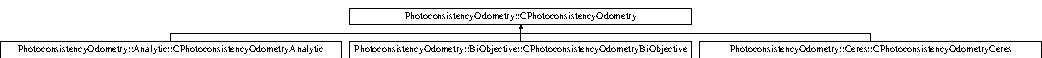
\includegraphics[height=0.779402cm]{class_photoconsistency_odometry_1_1_c_photoconsistency_odometry}
\end{center}
\end{figure}
\subsection*{Public Member Functions}
\begin{DoxyCompactItemize}
\item 
virtual void \hyperlink{class_photoconsistency_odometry_1_1_c_photoconsistency_odometry_a7464fc533b08dc7150eabd1086b84155}{setCameraMatrix} (Eigen::Matrix3f \&camMat)=0
\item 
virtual void \hyperlink{class_photoconsistency_odometry_1_1_c_photoconsistency_odometry_aa017bf63aeb6f3103d1b6fec8d38a888}{setSourceFrame} (cv::Mat \&imgGray, cv::Mat \&imgDepth)=0
\item 
virtual void \hyperlink{class_photoconsistency_odometry_1_1_c_photoconsistency_odometry_ac22e57f7f5039b7988447e7bd7d77f89}{setTargetFrame} (cv::Mat \&imgGray, cv::Mat \&imgDepth)=0
\item 
virtual void \hyperlink{class_photoconsistency_odometry_1_1_c_photoconsistency_odometry_a425e6bc2fbbc9dcf924ae197f5569ddf}{setInitialStateVector} (const std::vector$<$ double $>$ \&initialStateVector)=0
\item 
virtual void \hyperlink{class_photoconsistency_odometry_1_1_c_photoconsistency_odometry_aa7b0f04764e2c348556193281de58639}{optimize} ()=0
\item 
virtual void \hyperlink{class_photoconsistency_odometry_1_1_c_photoconsistency_odometry_a60e50c92161d1c2c1090757358ddba92}{getOptimalStateVector} (std::vector$<$ double $>$ \&optimalStateVector)=0
\item 
virtual void \hyperlink{class_photoconsistency_odometry_1_1_c_photoconsistency_odometry_a319f97afb21523fa6c66e9a04a607ea6}{getOptimalRigidTransformationMatrix} (Eigen::Matrix4f \&optimal\_\-Rt)=0
\end{DoxyCompactItemize}


\subsection{Detailed Description}
This abstract class defines the mandatory methods that any derived class must implement to compute the rigid (6DoF) transformation that best aligns a pair of RGBD frames using a photoconsistency maximization approach. 

\subsection{Member Function Documentation}
\hypertarget{class_photoconsistency_odometry_1_1_c_photoconsistency_odometry_a319f97afb21523fa6c66e9a04a607ea6}{
\index{PhotoconsistencyOdometry::CPhotoconsistencyOdometry@{PhotoconsistencyOdometry::CPhotoconsistencyOdometry}!getOptimalRigidTransformationMatrix@{getOptimalRigidTransformationMatrix}}
\index{getOptimalRigidTransformationMatrix@{getOptimalRigidTransformationMatrix}!PhotoconsistencyOdometry::CPhotoconsistencyOdometry@{PhotoconsistencyOdometry::CPhotoconsistencyOdometry}}
\subsubsection[{getOptimalRigidTransformationMatrix}]{\setlength{\rightskip}{0pt plus 5cm}virtual void PhotoconsistencyOdometry::CPhotoconsistencyOdometry::getOptimalRigidTransformationMatrix (
\begin{DoxyParamCaption}
\item[{Eigen::Matrix4f \&}]{optimal\_\-Rt}
\end{DoxyParamCaption}
)\hspace{0.3cm}{\ttfamily  \mbox{[}pure virtual\mbox{]}}}}
\label{class_photoconsistency_odometry_1_1_c_photoconsistency_odometry_a319f97afb21523fa6c66e9a04a607ea6}
Returns the optimal 4x4 rigid transformation matrix between the source and target frame. This method has to be called after calling the \hyperlink{class_photoconsistency_odometry_1_1_c_photoconsistency_odometry_aa7b0f04764e2c348556193281de58639}{optimize()} method. 

Implemented in \hyperlink{class_photoconsistency_odometry_1_1_analytic_1_1_c_photoconsistency_odometry_analytic_a48873715c3dc7a6ad8e8359d7c03254d}{PhotoconsistencyOdometry::Analytic::CPhotoconsistencyOdometryAnalytic}, \hyperlink{class_photoconsistency_odometry_1_1_bi_objective_1_1_c_photoconsistency_odometry_bi_objective_a1115655df7094d0566b786433fb0a223}{PhotoconsistencyOdometry::BiObjective::CPhotoconsistencyOdometryBiObjective}, and \hyperlink{class_photoconsistency_odometry_1_1_ceres_1_1_c_photoconsistency_odometry_ceres_aef03c06654345aeea7c0e128b575420d}{PhotoconsistencyOdometry::Ceres::CPhotoconsistencyOdometryCeres}.

\hypertarget{class_photoconsistency_odometry_1_1_c_photoconsistency_odometry_a60e50c92161d1c2c1090757358ddba92}{
\index{PhotoconsistencyOdometry::CPhotoconsistencyOdometry@{PhotoconsistencyOdometry::CPhotoconsistencyOdometry}!getOptimalStateVector@{getOptimalStateVector}}
\index{getOptimalStateVector@{getOptimalStateVector}!PhotoconsistencyOdometry::CPhotoconsistencyOdometry@{PhotoconsistencyOdometry::CPhotoconsistencyOdometry}}
\subsubsection[{getOptimalStateVector}]{\setlength{\rightskip}{0pt plus 5cm}virtual void PhotoconsistencyOdometry::CPhotoconsistencyOdometry::getOptimalStateVector (
\begin{DoxyParamCaption}
\item[{std::vector$<$ double $>$ \&}]{optimalStateVector}
\end{DoxyParamCaption}
)\hspace{0.3cm}{\ttfamily  \mbox{[}pure virtual\mbox{]}}}}
\label{class_photoconsistency_odometry_1_1_c_photoconsistency_odometry_a60e50c92161d1c2c1090757358ddba92}
Returns the optimal state vector. This method has to be called after calling the \hyperlink{class_photoconsistency_odometry_1_1_c_photoconsistency_odometry_aa7b0f04764e2c348556193281de58639}{optimize()} method. 

Implemented in \hyperlink{class_photoconsistency_odometry_1_1_analytic_1_1_c_photoconsistency_odometry_analytic_ad48c2851da3b626484d2d005b81d9b4e}{PhotoconsistencyOdometry::Analytic::CPhotoconsistencyOdometryAnalytic}, \hyperlink{class_photoconsistency_odometry_1_1_bi_objective_1_1_c_photoconsistency_odometry_bi_objective_acc57b9e6e38f85071f747d935023e7fd}{PhotoconsistencyOdometry::BiObjective::CPhotoconsistencyOdometryBiObjective}, and \hyperlink{class_photoconsistency_odometry_1_1_ceres_1_1_c_photoconsistency_odometry_ceres_a54f00adc07a9027430b4044284dec16c}{PhotoconsistencyOdometry::Ceres::CPhotoconsistencyOdometryCeres}.

\hypertarget{class_photoconsistency_odometry_1_1_c_photoconsistency_odometry_aa7b0f04764e2c348556193281de58639}{
\index{PhotoconsistencyOdometry::CPhotoconsistencyOdometry@{PhotoconsistencyOdometry::CPhotoconsistencyOdometry}!optimize@{optimize}}
\index{optimize@{optimize}!PhotoconsistencyOdometry::CPhotoconsistencyOdometry@{PhotoconsistencyOdometry::CPhotoconsistencyOdometry}}
\subsubsection[{optimize}]{\setlength{\rightskip}{0pt plus 5cm}virtual void PhotoconsistencyOdometry::CPhotoconsistencyOdometry::optimize (
\begin{DoxyParamCaption}
{}
\end{DoxyParamCaption}
)\hspace{0.3cm}{\ttfamily  \mbox{[}pure virtual\mbox{]}}}}
\label{class_photoconsistency_odometry_1_1_c_photoconsistency_odometry_aa7b0f04764e2c348556193281de58639}
Launches the least-\/squares optimization process to find the configuration of the state vector parameters that maximizes the photoconsistency between the source and target frame. 

Implemented in \hyperlink{class_photoconsistency_odometry_1_1_analytic_1_1_c_photoconsistency_odometry_analytic_aadf26b26688281cd18375984c1cc719e}{PhotoconsistencyOdometry::Analytic::CPhotoconsistencyOdometryAnalytic}, \hyperlink{class_photoconsistency_odometry_1_1_bi_objective_1_1_c_photoconsistency_odometry_bi_objective_a653474944f8cea88fc98074d3da4b551}{PhotoconsistencyOdometry::BiObjective::CPhotoconsistencyOdometryBiObjective}, and \hyperlink{class_photoconsistency_odometry_1_1_ceres_1_1_c_photoconsistency_odometry_ceres_af177ce6dd5517d73d5cf25da266a2777}{PhotoconsistencyOdometry::Ceres::CPhotoconsistencyOdometryCeres}.

\hypertarget{class_photoconsistency_odometry_1_1_c_photoconsistency_odometry_a7464fc533b08dc7150eabd1086b84155}{
\index{PhotoconsistencyOdometry::CPhotoconsistencyOdometry@{PhotoconsistencyOdometry::CPhotoconsistencyOdometry}!setCameraMatrix@{setCameraMatrix}}
\index{setCameraMatrix@{setCameraMatrix}!PhotoconsistencyOdometry::CPhotoconsistencyOdometry@{PhotoconsistencyOdometry::CPhotoconsistencyOdometry}}
\subsubsection[{setCameraMatrix}]{\setlength{\rightskip}{0pt plus 5cm}virtual void PhotoconsistencyOdometry::CPhotoconsistencyOdometry::setCameraMatrix (
\begin{DoxyParamCaption}
\item[{Eigen::Matrix3f \&}]{camMat}
\end{DoxyParamCaption}
)\hspace{0.3cm}{\ttfamily  \mbox{[}pure virtual\mbox{]}}}}
\label{class_photoconsistency_odometry_1_1_c_photoconsistency_odometry_a7464fc533b08dc7150eabd1086b84155}
Sets the 3x3 matrix of (pinhole) camera intrinsic parameters used to obtain the 3D colored point cloud from the RGB and depth images. 

Implemented in \hyperlink{class_photoconsistency_odometry_1_1_analytic_1_1_c_photoconsistency_odometry_analytic_af55a42286ff6f056ad33103dd7c3b0a9}{PhotoconsistencyOdometry::Analytic::CPhotoconsistencyOdometryAnalytic}, \hyperlink{class_photoconsistency_odometry_1_1_bi_objective_1_1_c_photoconsistency_odometry_bi_objective_a8f2e9f8a20c2496032577e5a7e50e506}{PhotoconsistencyOdometry::BiObjective::CPhotoconsistencyOdometryBiObjective}, and \hyperlink{class_photoconsistency_odometry_1_1_ceres_1_1_c_photoconsistency_odometry_ceres_ad45891d5065f3b00c40c8dbca794a632}{PhotoconsistencyOdometry::Ceres::CPhotoconsistencyOdometryCeres}.

\hypertarget{class_photoconsistency_odometry_1_1_c_photoconsistency_odometry_a425e6bc2fbbc9dcf924ae197f5569ddf}{
\index{PhotoconsistencyOdometry::CPhotoconsistencyOdometry@{PhotoconsistencyOdometry::CPhotoconsistencyOdometry}!setInitialStateVector@{setInitialStateVector}}
\index{setInitialStateVector@{setInitialStateVector}!PhotoconsistencyOdometry::CPhotoconsistencyOdometry@{PhotoconsistencyOdometry::CPhotoconsistencyOdometry}}
\subsubsection[{setInitialStateVector}]{\setlength{\rightskip}{0pt plus 5cm}virtual void PhotoconsistencyOdometry::CPhotoconsistencyOdometry::setInitialStateVector (
\begin{DoxyParamCaption}
\item[{const std::vector$<$ double $>$ \&}]{initialStateVector}
\end{DoxyParamCaption}
)\hspace{0.3cm}{\ttfamily  \mbox{[}pure virtual\mbox{]}}}}
\label{class_photoconsistency_odometry_1_1_c_photoconsistency_odometry_a425e6bc2fbbc9dcf924ae197f5569ddf}
Initializes the state vector to a certain value. The optimization process uses the initial state vector as the initial estimate. 

Implemented in \hyperlink{class_photoconsistency_odometry_1_1_analytic_1_1_c_photoconsistency_odometry_analytic_a6765ca12e063b199624e408fe07d2c13}{PhotoconsistencyOdometry::Analytic::CPhotoconsistencyOdometryAnalytic}, \hyperlink{class_photoconsistency_odometry_1_1_bi_objective_1_1_c_photoconsistency_odometry_bi_objective_a1e129e5db719ecf0365c40a09a26f9f0}{PhotoconsistencyOdometry::BiObjective::CPhotoconsistencyOdometryBiObjective}, and \hyperlink{class_photoconsistency_odometry_1_1_ceres_1_1_c_photoconsistency_odometry_ceres_a0993e83c820d16e606bce87edabbcd12}{PhotoconsistencyOdometry::Ceres::CPhotoconsistencyOdometryCeres}.

\hypertarget{class_photoconsistency_odometry_1_1_c_photoconsistency_odometry_aa017bf63aeb6f3103d1b6fec8d38a888}{
\index{PhotoconsistencyOdometry::CPhotoconsistencyOdometry@{PhotoconsistencyOdometry::CPhotoconsistencyOdometry}!setSourceFrame@{setSourceFrame}}
\index{setSourceFrame@{setSourceFrame}!PhotoconsistencyOdometry::CPhotoconsistencyOdometry@{PhotoconsistencyOdometry::CPhotoconsistencyOdometry}}
\subsubsection[{setSourceFrame}]{\setlength{\rightskip}{0pt plus 5cm}virtual void PhotoconsistencyOdometry::CPhotoconsistencyOdometry::setSourceFrame (
\begin{DoxyParamCaption}
\item[{cv::Mat \&}]{imgGray, }
\item[{cv::Mat \&}]{imgDepth}
\end{DoxyParamCaption}
)\hspace{0.3cm}{\ttfamily  \mbox{[}pure virtual\mbox{]}}}}
\label{class_photoconsistency_odometry_1_1_c_photoconsistency_odometry_aa017bf63aeb6f3103d1b6fec8d38a888}
Sets the source (Intensity+Depth) frame. 

Implemented in \hyperlink{class_photoconsistency_odometry_1_1_analytic_1_1_c_photoconsistency_odometry_analytic_a540df6929640bf7c1c248e27cc952772}{PhotoconsistencyOdometry::Analytic::CPhotoconsistencyOdometryAnalytic}, \hyperlink{class_photoconsistency_odometry_1_1_bi_objective_1_1_c_photoconsistency_odometry_bi_objective_acb6628a7f90ffd52798f61fdec55db0b}{PhotoconsistencyOdometry::BiObjective::CPhotoconsistencyOdometryBiObjective}, and \hyperlink{class_photoconsistency_odometry_1_1_ceres_1_1_c_photoconsistency_odometry_ceres_a987feeea7aab8dcc09ef82bde0814ed7}{PhotoconsistencyOdometry::Ceres::CPhotoconsistencyOdometryCeres}.

\hypertarget{class_photoconsistency_odometry_1_1_c_photoconsistency_odometry_ac22e57f7f5039b7988447e7bd7d77f89}{
\index{PhotoconsistencyOdometry::CPhotoconsistencyOdometry@{PhotoconsistencyOdometry::CPhotoconsistencyOdometry}!setTargetFrame@{setTargetFrame}}
\index{setTargetFrame@{setTargetFrame}!PhotoconsistencyOdometry::CPhotoconsistencyOdometry@{PhotoconsistencyOdometry::CPhotoconsistencyOdometry}}
\subsubsection[{setTargetFrame}]{\setlength{\rightskip}{0pt plus 5cm}virtual void PhotoconsistencyOdometry::CPhotoconsistencyOdometry::setTargetFrame (
\begin{DoxyParamCaption}
\item[{cv::Mat \&}]{imgGray, }
\item[{cv::Mat \&}]{imgDepth}
\end{DoxyParamCaption}
)\hspace{0.3cm}{\ttfamily  \mbox{[}pure virtual\mbox{]}}}}
\label{class_photoconsistency_odometry_1_1_c_photoconsistency_odometry_ac22e57f7f5039b7988447e7bd7d77f89}
Sets the source (Intensity+Depth) frame. 

Implemented in \hyperlink{class_photoconsistency_odometry_1_1_analytic_1_1_c_photoconsistency_odometry_analytic_a820824acdf3019f17ba889d0455e7f9c}{PhotoconsistencyOdometry::Analytic::CPhotoconsistencyOdometryAnalytic}, \hyperlink{class_photoconsistency_odometry_1_1_bi_objective_1_1_c_photoconsistency_odometry_bi_objective_ace2177b6d8081644465bad2b1fc4e176}{PhotoconsistencyOdometry::BiObjective::CPhotoconsistencyOdometryBiObjective}, and \hyperlink{class_photoconsistency_odometry_1_1_ceres_1_1_c_photoconsistency_odometry_ceres_afb707483f6766c5069eaad9824382272}{PhotoconsistencyOdometry::Ceres::CPhotoconsistencyOdometryCeres}.



The documentation for this class was generated from the following file:\begin{DoxyCompactItemize}
\item 
CPhotoconsistencyOdometry.h\end{DoxyCompactItemize}

\hypertarget{class_photoconsistency_odometry_1_1_analytic_1_1_c_photoconsistency_odometry_analytic}{
\section{PhotoconsistencyOdometry::Analytic::CPhotoconsistencyOdometryAnalytic Class Reference}
\label{class_photoconsistency_odometry_1_1_analytic_1_1_c_photoconsistency_odometry_analytic}\index{PhotoconsistencyOdometry::Analytic::CPhotoconsistencyOdometryAnalytic@{PhotoconsistencyOdometry::Analytic::CPhotoconsistencyOdometryAnalytic}}
}


{\ttfamily \#include $<$CPhotoconsistencyOdometryAnalytic.h$>$}

Inheritance diagram for PhotoconsistencyOdometry::Analytic::CPhotoconsistencyOdometryAnalytic:\begin{figure}[H]
\begin{center}
\leavevmode
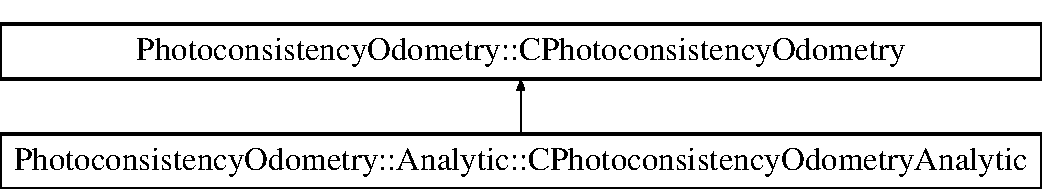
\includegraphics[height=2.000000cm]{class_photoconsistency_odometry_1_1_analytic_1_1_c_photoconsistency_odometry_analytic}
\end{center}
\end{figure}
\subsection*{Public Member Functions}
\begin{DoxyCompactItemize}
\item 
void \hyperlink{class_photoconsistency_odometry_1_1_analytic_1_1_c_photoconsistency_odometry_analytic_af473a25172cf498f50cec44b697f8e81}{setMinDepth} (float minD)
\item 
void \hyperlink{class_photoconsistency_odometry_1_1_analytic_1_1_c_photoconsistency_odometry_analytic_a5553935095782a68830efa1d4f4ccce5}{setMaxDepth} (float maxD)
\item 
void \hyperlink{class_photoconsistency_odometry_1_1_analytic_1_1_c_photoconsistency_odometry_analytic_af55a42286ff6f056ad33103dd7c3b0a9}{setCameraMatrix} (Eigen::Matrix3f \&camMat)
\item 
void \hyperlink{class_photoconsistency_odometry_1_1_analytic_1_1_c_photoconsistency_odometry_analytic_a540df6929640bf7c1c248e27cc952772}{setSourceFrame} (cv::Mat \&imgGray, cv::Mat \&imgDepth)
\item 
void \hyperlink{class_photoconsistency_odometry_1_1_analytic_1_1_c_photoconsistency_odometry_analytic_ac2f9288148db6b93b5cbe6a77818106d}{setTargetFrame} (cv::Mat \&imgGray)
\item 
void \hyperlink{class_photoconsistency_odometry_1_1_analytic_1_1_c_photoconsistency_odometry_analytic_a6765ca12e063b199624e408fe07d2c13}{setInitialStateVector} (const std::vector$<$ double $>$ \&initialStateVector)
\item 
void \hyperlink{class_photoconsistency_odometry_1_1_analytic_1_1_c_photoconsistency_odometry_analytic_aadf26b26688281cd18375984c1cc719e}{optimize} ()
\item 
void \hyperlink{class_photoconsistency_odometry_1_1_analytic_1_1_c_photoconsistency_odometry_analytic_ad48c2851da3b626484d2d005b81d9b4e}{getOptimalStateVector} (std::vector$<$ double $>$ \&optimalStateVector)
\item 
void \hyperlink{class_photoconsistency_odometry_1_1_analytic_1_1_c_photoconsistency_odometry_analytic_a48873715c3dc7a6ad8e8359d7c03254d}{getOptimalRigidTransformationMatrix} (Eigen::Matrix4f \&optimal\_\-Rt)
\item 
void \hyperlink{class_photoconsistency_odometry_1_1_analytic_1_1_c_photoconsistency_odometry_analytic_a96b148bbad6c72053fc93366bb0085d2}{readConfigurationFile} (std::string fileName)
\end{DoxyCompactItemize}
\subsection*{Private Types}
\begin{DoxyCompactItemize}
\item 
enum {\bfseries TerminationCriteriaType} \{ {\bfseries NonTerminated} =  -\/1, 
{\bfseries MaxIterationsReached} =  0, 
{\bfseries GradientNormLowerThanThreshold} =  1
 \}
\end{DoxyCompactItemize}
\subsection*{Private Member Functions}
\begin{DoxyCompactItemize}
\item 
\hypertarget{class_photoconsistency_odometry_1_1_analytic_1_1_c_photoconsistency_odometry_analytic_added156167e70927ad08b8c5f167aa7c}{
void {\bfseries buildPyramid} (cv::Mat \&img, std::vector$<$ cv::Mat $>$ \&pyramid, int levels, bool applyBlur)}
\label{class_photoconsistency_odometry_1_1_analytic_1_1_c_photoconsistency_odometry_analytic_added156167e70927ad08b8c5f167aa7c}

\item 
\hypertarget{class_photoconsistency_odometry_1_1_analytic_1_1_c_photoconsistency_odometry_analytic_a98cd69b765d58e68fb83d53e0a45944b}{
void {\bfseries buildDerivativesPyramids} (std::vector$<$ cv::Mat $>$ \&imagePyramid, std::vector$<$ cv::Mat $>$ \&derXPyramid, std::vector$<$ cv::Mat $>$ \&derYPyramid)}
\label{class_photoconsistency_odometry_1_1_analytic_1_1_c_photoconsistency_odometry_analytic_a98cd69b765d58e68fb83d53e0a45944b}

\item 
\hypertarget{class_photoconsistency_odometry_1_1_analytic_1_1_c_photoconsistency_odometry_analytic_a0de61bdb5fa8cf8840b908aa62bbc7ee}{
void {\bfseries computeResidualsAndJacobians} (cv::Mat \&source\_\-grayImg, cv::Mat \&source\_\-depthImg, cv::Mat \&target\_\-grayImg, cv::Mat \&target\_\-gradXImg, cv::Mat \&target\_\-gradYImg, Eigen::Matrix$<$ double, Eigen::Dynamic, 1 $>$ \&residuals, Eigen::Matrix$<$ double, Eigen::Dynamic, 6 $>$ \&jacobians, cv::Mat \&warped\_\-source\_\-grayImage)}
\label{class_photoconsistency_odometry_1_1_analytic_1_1_c_photoconsistency_odometry_analytic_a0de61bdb5fa8cf8840b908aa62bbc7ee}

\item 
\hypertarget{class_photoconsistency_odometry_1_1_analytic_1_1_c_photoconsistency_odometry_analytic_ae9a8a62f578082c2cba0b3919fa81673}{
bool {\bfseries testTerminationCriteria} ()}
\label{class_photoconsistency_odometry_1_1_analytic_1_1_c_photoconsistency_odometry_analytic_ae9a8a62f578082c2cba0b3919fa81673}

\end{DoxyCompactItemize}
\subsection*{Private Attributes}
\begin{DoxyCompactItemize}
\item 
std::vector$<$ cv::Mat $>$ \hyperlink{class_photoconsistency_odometry_1_1_analytic_1_1_c_photoconsistency_odometry_analytic_ab593c493a85a7a140a6f47fc89554793}{gray0Pyr}
\item 
\hypertarget{class_photoconsistency_odometry_1_1_analytic_1_1_c_photoconsistency_odometry_analytic_aca69c56d9dcce3d77b31a674b948d153}{
std::vector$<$ cv::Mat $>$ {\bfseries gray1Pyr}}
\label{class_photoconsistency_odometry_1_1_analytic_1_1_c_photoconsistency_odometry_analytic_aca69c56d9dcce3d77b31a674b948d153}

\item 
\hypertarget{class_photoconsistency_odometry_1_1_analytic_1_1_c_photoconsistency_odometry_analytic_abde99cb4532ee4df75325a99d273ccce}{
std::vector$<$ cv::Mat $>$ {\bfseries depth0Pyr}}
\label{class_photoconsistency_odometry_1_1_analytic_1_1_c_photoconsistency_odometry_analytic_abde99cb4532ee4df75325a99d273ccce}

\item 
\hypertarget{class_photoconsistency_odometry_1_1_analytic_1_1_c_photoconsistency_odometry_analytic_a6582703e8d0d1d9d2fb9c8a86e997dec}{
std::vector$<$ cv::Mat $>$ {\bfseries gray1GradXPyr}}
\label{class_photoconsistency_odometry_1_1_analytic_1_1_c_photoconsistency_odometry_analytic_a6582703e8d0d1d9d2fb9c8a86e997dec}

\item 
\hypertarget{class_photoconsistency_odometry_1_1_analytic_1_1_c_photoconsistency_odometry_analytic_aeb53b3a56274a6425562291eeda95af5}{
std::vector$<$ cv::Mat $>$ {\bfseries gray1GradYPyr}}
\label{class_photoconsistency_odometry_1_1_analytic_1_1_c_photoconsistency_odometry_analytic_aeb53b3a56274a6425562291eeda95af5}

\item 
Eigen::Matrix3f \hyperlink{class_photoconsistency_odometry_1_1_analytic_1_1_c_photoconsistency_odometry_analytic_a6338098cb3cee04a59768a27b84e29e0}{cameraMatrix}
\item 
int \hyperlink{class_photoconsistency_odometry_1_1_analytic_1_1_c_photoconsistency_odometry_analytic_a52b80772f2fabe73161055dc84ce2687}{optimizationLevel}
\item 
int \hyperlink{class_photoconsistency_odometry_1_1_analytic_1_1_c_photoconsistency_odometry_analytic_a23743290709f60c13f55b7a9664ae30d}{numOptimizationLevels}
\item 
std::vector$<$ float $>$ \hyperlink{class_photoconsistency_odometry_1_1_analytic_1_1_c_photoconsistency_odometry_analytic_a0c9b0540f2697f7b137b1a36ce3e2c18}{lambda\_\-optimization\_\-step}
\item 
std::vector$<$ int $>$ \hyperlink{class_photoconsistency_odometry_1_1_analytic_1_1_c_photoconsistency_odometry_analytic_abc3f7da046ef73b3cd4b8a4ad5abf441}{blurFilterSize}
\item 
std::vector$<$ float $>$ \hyperlink{class_photoconsistency_odometry_1_1_analytic_1_1_c_photoconsistency_odometry_analytic_adb99f12e7b9b1aa4b31b766b51e8a3c0}{imageGradientsScalingFactor}
\item 
std::vector$<$ int $>$ \hyperlink{class_photoconsistency_odometry_1_1_analytic_1_1_c_photoconsistency_odometry_analytic_ac84492170047058895b65f8b3f7d72a2}{max\_\-num\_\-iterations}
\item 
std::vector$<$ float $>$ \hyperlink{class_photoconsistency_odometry_1_1_analytic_1_1_c_photoconsistency_odometry_analytic_a0c34a8b704b2340114f16e98dcc33238}{min\_\-gradient\_\-norm}
\item 
bool \hyperlink{class_photoconsistency_odometry_1_1_analytic_1_1_c_photoconsistency_odometry_analytic_a100c9755e220fe7cc1cdba95211fb506}{visualizeIterations}
\item 
Eigen::Matrix$<$ double, 6, 1 $>$ \hyperlink{class_photoconsistency_odometry_1_1_analytic_1_1_c_photoconsistency_odometry_analytic_a46fc9664879ed9582eb173709fba3924}{stateVector}
\item 
Eigen::Matrix$<$ double, 6, 1 $>$ \hyperlink{class_photoconsistency_odometry_1_1_analytic_1_1_c_photoconsistency_odometry_analytic_ae1c72bf91edb0171331fb9c729dec27b}{gradients}
\item 
int \hyperlink{class_photoconsistency_odometry_1_1_analytic_1_1_c_photoconsistency_odometry_analytic_a8eea3326f2d11a5a30e53b171464ccb2}{iter}
\item 
float \hyperlink{class_photoconsistency_odometry_1_1_analytic_1_1_c_photoconsistency_odometry_analytic_a7b34e994ff1b81ae11e3211636045171}{minDepth}
\item 
float \hyperlink{class_photoconsistency_odometry_1_1_analytic_1_1_c_photoconsistency_odometry_analytic_a473668de10bebdfbd3c863cba5bf22c6}{maxDepth}
\end{DoxyCompactItemize}


\subsection{Detailed Description}
This class computes the rigid (6DoF) transformation that best aligns a pair of RGBD frames using a photoconsistency maximization approach. To estimate the rigid transformation, this class implements a coarse to fine approach. Thus, the algorithm starts finding a first pose approximation at a low resolution level and uses the estimate to initialize the optimization at greater image scales. Both the residuals and jacobians are computed analytically. 

\subsection{Member Function Documentation}
\hypertarget{class_photoconsistency_odometry_1_1_analytic_1_1_c_photoconsistency_odometry_analytic_a48873715c3dc7a6ad8e8359d7c03254d}{
\index{PhotoconsistencyOdometry::Analytic::CPhotoconsistencyOdometryAnalytic@{PhotoconsistencyOdometry::Analytic::CPhotoconsistencyOdometryAnalytic}!getOptimalRigidTransformationMatrix@{getOptimalRigidTransformationMatrix}}
\index{getOptimalRigidTransformationMatrix@{getOptimalRigidTransformationMatrix}!PhotoconsistencyOdometry::Analytic::CPhotoconsistencyOdometryAnalytic@{PhotoconsistencyOdometry::Analytic::CPhotoconsistencyOdometryAnalytic}}
\subsubsection[{getOptimalRigidTransformationMatrix}]{\setlength{\rightskip}{0pt plus 5cm}void PhotoconsistencyOdometry::Analytic::CPhotoconsistencyOdometryAnalytic::getOptimalRigidTransformationMatrix (
\begin{DoxyParamCaption}
\item[{Eigen::Matrix4f \&}]{optimal\_\-Rt}
\end{DoxyParamCaption}
)\hspace{0.3cm}{\ttfamily  \mbox{[}inline, virtual\mbox{]}}}}
\label{class_photoconsistency_odometry_1_1_analytic_1_1_c_photoconsistency_odometry_analytic_a48873715c3dc7a6ad8e8359d7c03254d}
Returns the optimal 4x4 rigid transformation matrix between the source and target frame. This method has to be called after calling the \hyperlink{class_photoconsistency_odometry_1_1_analytic_1_1_c_photoconsistency_odometry_analytic_aadf26b26688281cd18375984c1cc719e}{optimize()} method. 

Implements \hyperlink{class_photoconsistency_odometry_1_1_c_photoconsistency_odometry_a319f97afb21523fa6c66e9a04a607ea6}{PhotoconsistencyOdometry::CPhotoconsistencyOdometry}.

\hypertarget{class_photoconsistency_odometry_1_1_analytic_1_1_c_photoconsistency_odometry_analytic_ad48c2851da3b626484d2d005b81d9b4e}{
\index{PhotoconsistencyOdometry::Analytic::CPhotoconsistencyOdometryAnalytic@{PhotoconsistencyOdometry::Analytic::CPhotoconsistencyOdometryAnalytic}!getOptimalStateVector@{getOptimalStateVector}}
\index{getOptimalStateVector@{getOptimalStateVector}!PhotoconsistencyOdometry::Analytic::CPhotoconsistencyOdometryAnalytic@{PhotoconsistencyOdometry::Analytic::CPhotoconsistencyOdometryAnalytic}}
\subsubsection[{getOptimalStateVector}]{\setlength{\rightskip}{0pt plus 5cm}void PhotoconsistencyOdometry::Analytic::CPhotoconsistencyOdometryAnalytic::getOptimalStateVector (
\begin{DoxyParamCaption}
\item[{std::vector$<$ double $>$ \&}]{optimalStateVector}
\end{DoxyParamCaption}
)\hspace{0.3cm}{\ttfamily  \mbox{[}inline, virtual\mbox{]}}}}
\label{class_photoconsistency_odometry_1_1_analytic_1_1_c_photoconsistency_odometry_analytic_ad48c2851da3b626484d2d005b81d9b4e}
Returns the optimal state vector. This method has to be called after calling the \hyperlink{class_photoconsistency_odometry_1_1_analytic_1_1_c_photoconsistency_odometry_analytic_aadf26b26688281cd18375984c1cc719e}{optimize()} method. 

Implements \hyperlink{class_photoconsistency_odometry_1_1_c_photoconsistency_odometry_a60e50c92161d1c2c1090757358ddba92}{PhotoconsistencyOdometry::CPhotoconsistencyOdometry}.

\hypertarget{class_photoconsistency_odometry_1_1_analytic_1_1_c_photoconsistency_odometry_analytic_aadf26b26688281cd18375984c1cc719e}{
\index{PhotoconsistencyOdometry::Analytic::CPhotoconsistencyOdometryAnalytic@{PhotoconsistencyOdometry::Analytic::CPhotoconsistencyOdometryAnalytic}!optimize@{optimize}}
\index{optimize@{optimize}!PhotoconsistencyOdometry::Analytic::CPhotoconsistencyOdometryAnalytic@{PhotoconsistencyOdometry::Analytic::CPhotoconsistencyOdometryAnalytic}}
\subsubsection[{optimize}]{\setlength{\rightskip}{0pt plus 5cm}void PhotoconsistencyOdometry::Analytic::CPhotoconsistencyOdometryAnalytic::optimize (
\begin{DoxyParamCaption}
{}
\end{DoxyParamCaption}
)\hspace{0.3cm}{\ttfamily  \mbox{[}inline, virtual\mbox{]}}}}
\label{class_photoconsistency_odometry_1_1_analytic_1_1_c_photoconsistency_odometry_analytic_aadf26b26688281cd18375984c1cc719e}
Launches the least-\/squares optimization process to find the configuration of the state vector parameters that maximizes the photoconsistency between the source and target frame. 

Implements \hyperlink{class_photoconsistency_odometry_1_1_c_photoconsistency_odometry_aa7b0f04764e2c348556193281de58639}{PhotoconsistencyOdometry::CPhotoconsistencyOdometry}.

\hypertarget{class_photoconsistency_odometry_1_1_analytic_1_1_c_photoconsistency_odometry_analytic_a96b148bbad6c72053fc93366bb0085d2}{
\index{PhotoconsistencyOdometry::Analytic::CPhotoconsistencyOdometryAnalytic@{PhotoconsistencyOdometry::Analytic::CPhotoconsistencyOdometryAnalytic}!readConfigurationFile@{readConfigurationFile}}
\index{readConfigurationFile@{readConfigurationFile}!PhotoconsistencyOdometry::Analytic::CPhotoconsistencyOdometryAnalytic@{PhotoconsistencyOdometry::Analytic::CPhotoconsistencyOdometryAnalytic}}
\subsubsection[{readConfigurationFile}]{\setlength{\rightskip}{0pt plus 5cm}void PhotoconsistencyOdometry::Analytic::CPhotoconsistencyOdometryAnalytic::readConfigurationFile (
\begin{DoxyParamCaption}
\item[{std::string}]{fileName}
\end{DoxyParamCaption}
)\hspace{0.3cm}{\ttfamily  \mbox{[}inline\mbox{]}}}}
\label{class_photoconsistency_odometry_1_1_analytic_1_1_c_photoconsistency_odometry_analytic_a96b148bbad6c72053fc93366bb0085d2}
Reads the configuration parameters from a .yml file. \hypertarget{class_photoconsistency_odometry_1_1_analytic_1_1_c_photoconsistency_odometry_analytic_af55a42286ff6f056ad33103dd7c3b0a9}{
\index{PhotoconsistencyOdometry::Analytic::CPhotoconsistencyOdometryAnalytic@{PhotoconsistencyOdometry::Analytic::CPhotoconsistencyOdometryAnalytic}!setCameraMatrix@{setCameraMatrix}}
\index{setCameraMatrix@{setCameraMatrix}!PhotoconsistencyOdometry::Analytic::CPhotoconsistencyOdometryAnalytic@{PhotoconsistencyOdometry::Analytic::CPhotoconsistencyOdometryAnalytic}}
\subsubsection[{setCameraMatrix}]{\setlength{\rightskip}{0pt plus 5cm}void PhotoconsistencyOdometry::Analytic::CPhotoconsistencyOdometryAnalytic::setCameraMatrix (
\begin{DoxyParamCaption}
\item[{Eigen::Matrix3f \&}]{camMat}
\end{DoxyParamCaption}
)\hspace{0.3cm}{\ttfamily  \mbox{[}inline, virtual\mbox{]}}}}
\label{class_photoconsistency_odometry_1_1_analytic_1_1_c_photoconsistency_odometry_analytic_af55a42286ff6f056ad33103dd7c3b0a9}
Sets the 3x3 matrix of (pinhole) camera intrinsic parameters used to obtain the 3D colored point cloud from the RGB and depth images. 

Implements \hyperlink{class_photoconsistency_odometry_1_1_c_photoconsistency_odometry_a7464fc533b08dc7150eabd1086b84155}{PhotoconsistencyOdometry::CPhotoconsistencyOdometry}.

\hypertarget{class_photoconsistency_odometry_1_1_analytic_1_1_c_photoconsistency_odometry_analytic_a6765ca12e063b199624e408fe07d2c13}{
\index{PhotoconsistencyOdometry::Analytic::CPhotoconsistencyOdometryAnalytic@{PhotoconsistencyOdometry::Analytic::CPhotoconsistencyOdometryAnalytic}!setInitialStateVector@{setInitialStateVector}}
\index{setInitialStateVector@{setInitialStateVector}!PhotoconsistencyOdometry::Analytic::CPhotoconsistencyOdometryAnalytic@{PhotoconsistencyOdometry::Analytic::CPhotoconsistencyOdometryAnalytic}}
\subsubsection[{setInitialStateVector}]{\setlength{\rightskip}{0pt plus 5cm}void PhotoconsistencyOdometry::Analytic::CPhotoconsistencyOdometryAnalytic::setInitialStateVector (
\begin{DoxyParamCaption}
\item[{const std::vector$<$ double $>$ \&}]{initialStateVector}
\end{DoxyParamCaption}
)\hspace{0.3cm}{\ttfamily  \mbox{[}inline, virtual\mbox{]}}}}
\label{class_photoconsistency_odometry_1_1_analytic_1_1_c_photoconsistency_odometry_analytic_a6765ca12e063b199624e408fe07d2c13}
Initializes the state vector to a certain value. The optimization process uses the initial state vector as the initial estimate. 

Implements \hyperlink{class_photoconsistency_odometry_1_1_c_photoconsistency_odometry_a425e6bc2fbbc9dcf924ae197f5569ddf}{PhotoconsistencyOdometry::CPhotoconsistencyOdometry}.

\hypertarget{class_photoconsistency_odometry_1_1_analytic_1_1_c_photoconsistency_odometry_analytic_a5553935095782a68830efa1d4f4ccce5}{
\index{PhotoconsistencyOdometry::Analytic::CPhotoconsistencyOdometryAnalytic@{PhotoconsistencyOdometry::Analytic::CPhotoconsistencyOdometryAnalytic}!setMaxDepth@{setMaxDepth}}
\index{setMaxDepth@{setMaxDepth}!PhotoconsistencyOdometry::Analytic::CPhotoconsistencyOdometryAnalytic@{PhotoconsistencyOdometry::Analytic::CPhotoconsistencyOdometryAnalytic}}
\subsubsection[{setMaxDepth}]{\setlength{\rightskip}{0pt plus 5cm}void PhotoconsistencyOdometry::Analytic::CPhotoconsistencyOdometryAnalytic::setMaxDepth (
\begin{DoxyParamCaption}
\item[{float}]{maxD}
\end{DoxyParamCaption}
)\hspace{0.3cm}{\ttfamily  \mbox{[}inline\mbox{]}}}}
\label{class_photoconsistency_odometry_1_1_analytic_1_1_c_photoconsistency_odometry_analytic_a5553935095782a68830efa1d4f4ccce5}
Sets the maximum depth distance (m) to consider a certain pixel valid. \hypertarget{class_photoconsistency_odometry_1_1_analytic_1_1_c_photoconsistency_odometry_analytic_af473a25172cf498f50cec44b697f8e81}{
\index{PhotoconsistencyOdometry::Analytic::CPhotoconsistencyOdometryAnalytic@{PhotoconsistencyOdometry::Analytic::CPhotoconsistencyOdometryAnalytic}!setMinDepth@{setMinDepth}}
\index{setMinDepth@{setMinDepth}!PhotoconsistencyOdometry::Analytic::CPhotoconsistencyOdometryAnalytic@{PhotoconsistencyOdometry::Analytic::CPhotoconsistencyOdometryAnalytic}}
\subsubsection[{setMinDepth}]{\setlength{\rightskip}{0pt plus 5cm}void PhotoconsistencyOdometry::Analytic::CPhotoconsistencyOdometryAnalytic::setMinDepth (
\begin{DoxyParamCaption}
\item[{float}]{minD}
\end{DoxyParamCaption}
)\hspace{0.3cm}{\ttfamily  \mbox{[}inline\mbox{]}}}}
\label{class_photoconsistency_odometry_1_1_analytic_1_1_c_photoconsistency_odometry_analytic_af473a25172cf498f50cec44b697f8e81}
Sets the minimum depth distance (m) to consider a certain pixel valid. \hypertarget{class_photoconsistency_odometry_1_1_analytic_1_1_c_photoconsistency_odometry_analytic_a540df6929640bf7c1c248e27cc952772}{
\index{PhotoconsistencyOdometry::Analytic::CPhotoconsistencyOdometryAnalytic@{PhotoconsistencyOdometry::Analytic::CPhotoconsistencyOdometryAnalytic}!setSourceFrame@{setSourceFrame}}
\index{setSourceFrame@{setSourceFrame}!PhotoconsistencyOdometry::Analytic::CPhotoconsistencyOdometryAnalytic@{PhotoconsistencyOdometry::Analytic::CPhotoconsistencyOdometryAnalytic}}
\subsubsection[{setSourceFrame}]{\setlength{\rightskip}{0pt plus 5cm}void PhotoconsistencyOdometry::Analytic::CPhotoconsistencyOdometryAnalytic::setSourceFrame (
\begin{DoxyParamCaption}
\item[{cv::Mat \&}]{imgGray, }
\item[{cv::Mat \&}]{imgDepth}
\end{DoxyParamCaption}
)\hspace{0.3cm}{\ttfamily  \mbox{[}inline, virtual\mbox{]}}}}
\label{class_photoconsistency_odometry_1_1_analytic_1_1_c_photoconsistency_odometry_analytic_a540df6929640bf7c1c248e27cc952772}
Sets the source (Intensity+Depth) frame. 

Implements \hyperlink{class_photoconsistency_odometry_1_1_c_photoconsistency_odometry_aa017bf63aeb6f3103d1b6fec8d38a888}{PhotoconsistencyOdometry::CPhotoconsistencyOdometry}.

\hypertarget{class_photoconsistency_odometry_1_1_analytic_1_1_c_photoconsistency_odometry_analytic_ac2f9288148db6b93b5cbe6a77818106d}{
\index{PhotoconsistencyOdometry::Analytic::CPhotoconsistencyOdometryAnalytic@{PhotoconsistencyOdometry::Analytic::CPhotoconsistencyOdometryAnalytic}!setTargetFrame@{setTargetFrame}}
\index{setTargetFrame@{setTargetFrame}!PhotoconsistencyOdometry::Analytic::CPhotoconsistencyOdometryAnalytic@{PhotoconsistencyOdometry::Analytic::CPhotoconsistencyOdometryAnalytic}}
\subsubsection[{setTargetFrame}]{\setlength{\rightskip}{0pt plus 5cm}void PhotoconsistencyOdometry::Analytic::CPhotoconsistencyOdometryAnalytic::setTargetFrame (
\begin{DoxyParamCaption}
\item[{cv::Mat \&}]{imgGray}
\end{DoxyParamCaption}
)\hspace{0.3cm}{\ttfamily  \mbox{[}inline, virtual\mbox{]}}}}
\label{class_photoconsistency_odometry_1_1_analytic_1_1_c_photoconsistency_odometry_analytic_ac2f9288148db6b93b5cbe6a77818106d}
Sets the target intensity frame. 

Implements \hyperlink{class_photoconsistency_odometry_1_1_c_photoconsistency_odometry_a4f04b88ac54670b03b5c2bf773bca018}{PhotoconsistencyOdometry::CPhotoconsistencyOdometry}.



\subsection{Field Documentation}
\hypertarget{class_photoconsistency_odometry_1_1_analytic_1_1_c_photoconsistency_odometry_analytic_abc3f7da046ef73b3cd4b8a4ad5abf441}{
\index{PhotoconsistencyOdometry::Analytic::CPhotoconsistencyOdometryAnalytic@{PhotoconsistencyOdometry::Analytic::CPhotoconsistencyOdometryAnalytic}!blurFilterSize@{blurFilterSize}}
\index{blurFilterSize@{blurFilterSize}!PhotoconsistencyOdometry::Analytic::CPhotoconsistencyOdometryAnalytic@{PhotoconsistencyOdometry::Analytic::CPhotoconsistencyOdometryAnalytic}}
\subsubsection[{blurFilterSize}]{\setlength{\rightskip}{0pt plus 5cm}std::vector$<$int$>$ {\bf PhotoconsistencyOdometry::Analytic::CPhotoconsistencyOdometryAnalytic::blurFilterSize}\hspace{0.3cm}{\ttfamily  \mbox{[}private\mbox{]}}}}
\label{class_photoconsistency_odometry_1_1_analytic_1_1_c_photoconsistency_odometry_analytic_abc3f7da046ef73b3cd4b8a4ad5abf441}
Size (in pixels) of the blur filter (at each level). \hypertarget{class_photoconsistency_odometry_1_1_analytic_1_1_c_photoconsistency_odometry_analytic_a6338098cb3cee04a59768a27b84e29e0}{
\index{PhotoconsistencyOdometry::Analytic::CPhotoconsistencyOdometryAnalytic@{PhotoconsistencyOdometry::Analytic::CPhotoconsistencyOdometryAnalytic}!cameraMatrix@{cameraMatrix}}
\index{cameraMatrix@{cameraMatrix}!PhotoconsistencyOdometry::Analytic::CPhotoconsistencyOdometryAnalytic@{PhotoconsistencyOdometry::Analytic::CPhotoconsistencyOdometryAnalytic}}
\subsubsection[{cameraMatrix}]{\setlength{\rightskip}{0pt plus 5cm}Eigen::Matrix3f {\bf PhotoconsistencyOdometry::Analytic::CPhotoconsistencyOdometryAnalytic::cameraMatrix}\hspace{0.3cm}{\ttfamily  \mbox{[}private\mbox{]}}}}
\label{class_photoconsistency_odometry_1_1_analytic_1_1_c_photoconsistency_odometry_analytic_a6338098cb3cee04a59768a27b84e29e0}
Camera matrix (intrinsic parameters). \hypertarget{class_photoconsistency_odometry_1_1_analytic_1_1_c_photoconsistency_odometry_analytic_ae1c72bf91edb0171331fb9c729dec27b}{
\index{PhotoconsistencyOdometry::Analytic::CPhotoconsistencyOdometryAnalytic@{PhotoconsistencyOdometry::Analytic::CPhotoconsistencyOdometryAnalytic}!gradients@{gradients}}
\index{gradients@{gradients}!PhotoconsistencyOdometry::Analytic::CPhotoconsistencyOdometryAnalytic@{PhotoconsistencyOdometry::Analytic::CPhotoconsistencyOdometryAnalytic}}
\subsubsection[{gradients}]{\setlength{\rightskip}{0pt plus 5cm}Eigen::Matrix$<$double,6,1$>$ {\bf PhotoconsistencyOdometry::Analytic::CPhotoconsistencyOdometryAnalytic::gradients}\hspace{0.3cm}{\ttfamily  \mbox{[}private\mbox{]}}}}
\label{class_photoconsistency_odometry_1_1_analytic_1_1_c_photoconsistency_odometry_analytic_ae1c72bf91edb0171331fb9c729dec27b}
Gradient of the error function. \hypertarget{class_photoconsistency_odometry_1_1_analytic_1_1_c_photoconsistency_odometry_analytic_ab593c493a85a7a140a6f47fc89554793}{
\index{PhotoconsistencyOdometry::Analytic::CPhotoconsistencyOdometryAnalytic@{PhotoconsistencyOdometry::Analytic::CPhotoconsistencyOdometryAnalytic}!gray0Pyr@{gray0Pyr}}
\index{gray0Pyr@{gray0Pyr}!PhotoconsistencyOdometry::Analytic::CPhotoconsistencyOdometryAnalytic@{PhotoconsistencyOdometry::Analytic::CPhotoconsistencyOdometryAnalytic}}
\subsubsection[{gray0Pyr}]{\setlength{\rightskip}{0pt plus 5cm}std::vector$<$cv::Mat$>$ {\bf PhotoconsistencyOdometry::Analytic::CPhotoconsistencyOdometryAnalytic::gray0Pyr}\hspace{0.3cm}{\ttfamily  \mbox{[}private\mbox{]}}}}
\label{class_photoconsistency_odometry_1_1_analytic_1_1_c_photoconsistency_odometry_analytic_ab593c493a85a7a140a6f47fc89554793}
Intensity (gray), depth and gradient image pyramids. Each pyramid has 'numOptimizationLevels' levels. \hypertarget{class_photoconsistency_odometry_1_1_analytic_1_1_c_photoconsistency_odometry_analytic_adb99f12e7b9b1aa4b31b766b51e8a3c0}{
\index{PhotoconsistencyOdometry::Analytic::CPhotoconsistencyOdometryAnalytic@{PhotoconsistencyOdometry::Analytic::CPhotoconsistencyOdometryAnalytic}!imageGradientsScalingFactor@{imageGradientsScalingFactor}}
\index{imageGradientsScalingFactor@{imageGradientsScalingFactor}!PhotoconsistencyOdometry::Analytic::CPhotoconsistencyOdometryAnalytic@{PhotoconsistencyOdometry::Analytic::CPhotoconsistencyOdometryAnalytic}}
\subsubsection[{imageGradientsScalingFactor}]{\setlength{\rightskip}{0pt plus 5cm}std::vector$<$float$>$ {\bf PhotoconsistencyOdometry::Analytic::CPhotoconsistencyOdometryAnalytic::imageGradientsScalingFactor}\hspace{0.3cm}{\ttfamily  \mbox{[}private\mbox{]}}}}
\label{class_photoconsistency_odometry_1_1_analytic_1_1_c_photoconsistency_odometry_analytic_adb99f12e7b9b1aa4b31b766b51e8a3c0}
Scaling factor applied to the image gradients (at each level). \hypertarget{class_photoconsistency_odometry_1_1_analytic_1_1_c_photoconsistency_odometry_analytic_a8eea3326f2d11a5a30e53b171464ccb2}{
\index{PhotoconsistencyOdometry::Analytic::CPhotoconsistencyOdometryAnalytic@{PhotoconsistencyOdometry::Analytic::CPhotoconsistencyOdometryAnalytic}!iter@{iter}}
\index{iter@{iter}!PhotoconsistencyOdometry::Analytic::CPhotoconsistencyOdometryAnalytic@{PhotoconsistencyOdometry::Analytic::CPhotoconsistencyOdometryAnalytic}}
\subsubsection[{iter}]{\setlength{\rightskip}{0pt plus 5cm}int {\bf PhotoconsistencyOdometry::Analytic::CPhotoconsistencyOdometryAnalytic::iter}\hspace{0.3cm}{\ttfamily  \mbox{[}private\mbox{]}}}}
\label{class_photoconsistency_odometry_1_1_analytic_1_1_c_photoconsistency_odometry_analytic_a8eea3326f2d11a5a30e53b171464ccb2}
Current iteration at the current optimization level. \hypertarget{class_photoconsistency_odometry_1_1_analytic_1_1_c_photoconsistency_odometry_analytic_a0c9b0540f2697f7b137b1a36ce3e2c18}{
\index{PhotoconsistencyOdometry::Analytic::CPhotoconsistencyOdometryAnalytic@{PhotoconsistencyOdometry::Analytic::CPhotoconsistencyOdometryAnalytic}!lambda\_\-optimization\_\-step@{lambda\_\-optimization\_\-step}}
\index{lambda\_\-optimization\_\-step@{lambda\_\-optimization\_\-step}!PhotoconsistencyOdometry::Analytic::CPhotoconsistencyOdometryAnalytic@{PhotoconsistencyOdometry::Analytic::CPhotoconsistencyOdometryAnalytic}}
\subsubsection[{lambda\_\-optimization\_\-step}]{\setlength{\rightskip}{0pt plus 5cm}std::vector$<$float$>$ {\bf PhotoconsistencyOdometry::Analytic::CPhotoconsistencyOdometryAnalytic::lambda\_\-optimization\_\-step}\hspace{0.3cm}{\ttfamily  \mbox{[}private\mbox{]}}}}
\label{class_photoconsistency_odometry_1_1_analytic_1_1_c_photoconsistency_odometry_analytic_a0c9b0540f2697f7b137b1a36ce3e2c18}
Scaling factor to update the state vector (at each level). \hypertarget{class_photoconsistency_odometry_1_1_analytic_1_1_c_photoconsistency_odometry_analytic_ac84492170047058895b65f8b3f7d72a2}{
\index{PhotoconsistencyOdometry::Analytic::CPhotoconsistencyOdometryAnalytic@{PhotoconsistencyOdometry::Analytic::CPhotoconsistencyOdometryAnalytic}!max\_\-num\_\-iterations@{max\_\-num\_\-iterations}}
\index{max\_\-num\_\-iterations@{max\_\-num\_\-iterations}!PhotoconsistencyOdometry::Analytic::CPhotoconsistencyOdometryAnalytic@{PhotoconsistencyOdometry::Analytic::CPhotoconsistencyOdometryAnalytic}}
\subsubsection[{max\_\-num\_\-iterations}]{\setlength{\rightskip}{0pt plus 5cm}std::vector$<$int$>$ {\bf PhotoconsistencyOdometry::Analytic::CPhotoconsistencyOdometryAnalytic::max\_\-num\_\-iterations}\hspace{0.3cm}{\ttfamily  \mbox{[}private\mbox{]}}}}
\label{class_photoconsistency_odometry_1_1_analytic_1_1_c_photoconsistency_odometry_analytic_ac84492170047058895b65f8b3f7d72a2}
Maximum number of iterations for the Gauss-\/Newton algorithm (at each level). \hypertarget{class_photoconsistency_odometry_1_1_analytic_1_1_c_photoconsistency_odometry_analytic_a473668de10bebdfbd3c863cba5bf22c6}{
\index{PhotoconsistencyOdometry::Analytic::CPhotoconsistencyOdometryAnalytic@{PhotoconsistencyOdometry::Analytic::CPhotoconsistencyOdometryAnalytic}!maxDepth@{maxDepth}}
\index{maxDepth@{maxDepth}!PhotoconsistencyOdometry::Analytic::CPhotoconsistencyOdometryAnalytic@{PhotoconsistencyOdometry::Analytic::CPhotoconsistencyOdometryAnalytic}}
\subsubsection[{maxDepth}]{\setlength{\rightskip}{0pt plus 5cm}float {\bf PhotoconsistencyOdometry::Analytic::CPhotoconsistencyOdometryAnalytic::maxDepth}\hspace{0.3cm}{\ttfamily  \mbox{[}private\mbox{]}}}}
\label{class_photoconsistency_odometry_1_1_analytic_1_1_c_photoconsistency_odometry_analytic_a473668de10bebdfbd3c863cba5bf22c6}
Maximum allowed depth to consider a depth pixel valid. \hypertarget{class_photoconsistency_odometry_1_1_analytic_1_1_c_photoconsistency_odometry_analytic_a0c34a8b704b2340114f16e98dcc33238}{
\index{PhotoconsistencyOdometry::Analytic::CPhotoconsistencyOdometryAnalytic@{PhotoconsistencyOdometry::Analytic::CPhotoconsistencyOdometryAnalytic}!min\_\-gradient\_\-norm@{min\_\-gradient\_\-norm}}
\index{min\_\-gradient\_\-norm@{min\_\-gradient\_\-norm}!PhotoconsistencyOdometry::Analytic::CPhotoconsistencyOdometryAnalytic@{PhotoconsistencyOdometry::Analytic::CPhotoconsistencyOdometryAnalytic}}
\subsubsection[{min\_\-gradient\_\-norm}]{\setlength{\rightskip}{0pt plus 5cm}std::vector$<$float$>$ {\bf PhotoconsistencyOdometry::Analytic::CPhotoconsistencyOdometryAnalytic::min\_\-gradient\_\-norm}\hspace{0.3cm}{\ttfamily  \mbox{[}private\mbox{]}}}}
\label{class_photoconsistency_odometry_1_1_analytic_1_1_c_photoconsistency_odometry_analytic_a0c34a8b704b2340114f16e98dcc33238}
Minimum gradient norm of the jacobian (at each level). \hypertarget{class_photoconsistency_odometry_1_1_analytic_1_1_c_photoconsistency_odometry_analytic_a7b34e994ff1b81ae11e3211636045171}{
\index{PhotoconsistencyOdometry::Analytic::CPhotoconsistencyOdometryAnalytic@{PhotoconsistencyOdometry::Analytic::CPhotoconsistencyOdometryAnalytic}!minDepth@{minDepth}}
\index{minDepth@{minDepth}!PhotoconsistencyOdometry::Analytic::CPhotoconsistencyOdometryAnalytic@{PhotoconsistencyOdometry::Analytic::CPhotoconsistencyOdometryAnalytic}}
\subsubsection[{minDepth}]{\setlength{\rightskip}{0pt plus 5cm}float {\bf PhotoconsistencyOdometry::Analytic::CPhotoconsistencyOdometryAnalytic::minDepth}\hspace{0.3cm}{\ttfamily  \mbox{[}private\mbox{]}}}}
\label{class_photoconsistency_odometry_1_1_analytic_1_1_c_photoconsistency_odometry_analytic_a7b34e994ff1b81ae11e3211636045171}
Minimum allowed depth to consider a depth pixel valid. \hypertarget{class_photoconsistency_odometry_1_1_analytic_1_1_c_photoconsistency_odometry_analytic_a23743290709f60c13f55b7a9664ae30d}{
\index{PhotoconsistencyOdometry::Analytic::CPhotoconsistencyOdometryAnalytic@{PhotoconsistencyOdometry::Analytic::CPhotoconsistencyOdometryAnalytic}!numOptimizationLevels@{numOptimizationLevels}}
\index{numOptimizationLevels@{numOptimizationLevels}!PhotoconsistencyOdometry::Analytic::CPhotoconsistencyOdometryAnalytic@{PhotoconsistencyOdometry::Analytic::CPhotoconsistencyOdometryAnalytic}}
\subsubsection[{numOptimizationLevels}]{\setlength{\rightskip}{0pt plus 5cm}int {\bf PhotoconsistencyOdometry::Analytic::CPhotoconsistencyOdometryAnalytic::numOptimizationLevels}\hspace{0.3cm}{\ttfamily  \mbox{[}private\mbox{]}}}}
\label{class_photoconsistency_odometry_1_1_analytic_1_1_c_photoconsistency_odometry_analytic_a23743290709f60c13f55b7a9664ae30d}
Number of optimization levels. \hypertarget{class_photoconsistency_odometry_1_1_analytic_1_1_c_photoconsistency_odometry_analytic_a52b80772f2fabe73161055dc84ce2687}{
\index{PhotoconsistencyOdometry::Analytic::CPhotoconsistencyOdometryAnalytic@{PhotoconsistencyOdometry::Analytic::CPhotoconsistencyOdometryAnalytic}!optimizationLevel@{optimizationLevel}}
\index{optimizationLevel@{optimizationLevel}!PhotoconsistencyOdometry::Analytic::CPhotoconsistencyOdometryAnalytic@{PhotoconsistencyOdometry::Analytic::CPhotoconsistencyOdometryAnalytic}}
\subsubsection[{optimizationLevel}]{\setlength{\rightskip}{0pt plus 5cm}int {\bf PhotoconsistencyOdometry::Analytic::CPhotoconsistencyOdometryAnalytic::optimizationLevel}\hspace{0.3cm}{\ttfamily  \mbox{[}private\mbox{]}}}}
\label{class_photoconsistency_odometry_1_1_analytic_1_1_c_photoconsistency_odometry_analytic_a52b80772f2fabe73161055dc84ce2687}
Current optimization level. Level 0 corresponds to the higher image resolution. \hypertarget{class_photoconsistency_odometry_1_1_analytic_1_1_c_photoconsistency_odometry_analytic_a46fc9664879ed9582eb173709fba3924}{
\index{PhotoconsistencyOdometry::Analytic::CPhotoconsistencyOdometryAnalytic@{PhotoconsistencyOdometry::Analytic::CPhotoconsistencyOdometryAnalytic}!stateVector@{stateVector}}
\index{stateVector@{stateVector}!PhotoconsistencyOdometry::Analytic::CPhotoconsistencyOdometryAnalytic@{PhotoconsistencyOdometry::Analytic::CPhotoconsistencyOdometryAnalytic}}
\subsubsection[{stateVector}]{\setlength{\rightskip}{0pt plus 5cm}Eigen::Matrix$<$double,6,1$>$ {\bf PhotoconsistencyOdometry::Analytic::CPhotoconsistencyOdometryAnalytic::stateVector}\hspace{0.3cm}{\ttfamily  \mbox{[}private\mbox{]}}}}
\label{class_photoconsistency_odometry_1_1_analytic_1_1_c_photoconsistency_odometry_analytic_a46fc9664879ed9582eb173709fba3924}
State vector. \hypertarget{class_photoconsistency_odometry_1_1_analytic_1_1_c_photoconsistency_odometry_analytic_a100c9755e220fe7cc1cdba95211fb506}{
\index{PhotoconsistencyOdometry::Analytic::CPhotoconsistencyOdometryAnalytic@{PhotoconsistencyOdometry::Analytic::CPhotoconsistencyOdometryAnalytic}!visualizeIterations@{visualizeIterations}}
\index{visualizeIterations@{visualizeIterations}!PhotoconsistencyOdometry::Analytic::CPhotoconsistencyOdometryAnalytic@{PhotoconsistencyOdometry::Analytic::CPhotoconsistencyOdometryAnalytic}}
\subsubsection[{visualizeIterations}]{\setlength{\rightskip}{0pt plus 5cm}bool {\bf PhotoconsistencyOdometry::Analytic::CPhotoconsistencyOdometryAnalytic::visualizeIterations}\hspace{0.3cm}{\ttfamily  \mbox{[}private\mbox{]}}}}
\label{class_photoconsistency_odometry_1_1_analytic_1_1_c_photoconsistency_odometry_analytic_a100c9755e220fe7cc1cdba95211fb506}
Enable the visualization of the optimization process (only for debug). 

The documentation for this class was generated from the following file:\begin{DoxyCompactItemize}
\item 
CPhotoconsistencyOdometryAnalytic.h\end{DoxyCompactItemize}

\hypertarget{class_photoconsistency_odometry_1_1_ceres_1_1_c_photoconsistency_odometry_ceres}{
\section{PhotoconsistencyOdometry::Ceres::CPhotoconsistencyOdometryCeres Class Reference}
\label{class_photoconsistency_odometry_1_1_ceres_1_1_c_photoconsistency_odometry_ceres}\index{PhotoconsistencyOdometry::Ceres::CPhotoconsistencyOdometryCeres@{PhotoconsistencyOdometry::Ceres::CPhotoconsistencyOdometryCeres}}
}


{\ttfamily \#include $<$CPhotoconsistencyOdometryCeres.h$>$}

Inheritance diagram for PhotoconsistencyOdometry::Ceres::CPhotoconsistencyOdometryCeres:\begin{figure}[H]
\begin{center}
\leavevmode
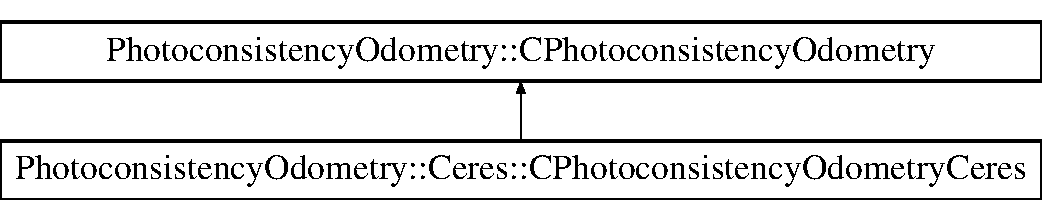
\includegraphics[height=2.000000cm]{class_photoconsistency_odometry_1_1_ceres_1_1_c_photoconsistency_odometry_ceres}
\end{center}
\end{figure}
\subsection*{Data Structures}
\begin{DoxyCompactItemize}
\item 
class \hyperlink{class_photoconsistency_odometry_1_1_ceres_1_1_c_photoconsistency_odometry_ceres_1_1_residual_r_g_b_d_photoconsistency}{ResidualRGBDPhotoconsistency}
\item 
class \hyperlink{class_photoconsistency_odometry_1_1_ceres_1_1_c_photoconsistency_odometry_ceres_1_1_visualization_callback}{VisualizationCallback}
\end{DoxyCompactItemize}
\subsection*{Public Member Functions}
\begin{DoxyCompactItemize}
\item 
void \hyperlink{class_photoconsistency_odometry_1_1_ceres_1_1_c_photoconsistency_odometry_ceres_ad45891d5065f3b00c40c8dbca794a632}{setCameraMatrix} (Eigen::Matrix3f \&camMat)
\item 
void \hyperlink{class_photoconsistency_odometry_1_1_ceres_1_1_c_photoconsistency_odometry_ceres_a987feeea7aab8dcc09ef82bde0814ed7}{setSourceFrame} (cv::Mat \&imgGray, cv::Mat \&imgDepth)
\item 
void \hyperlink{class_photoconsistency_odometry_1_1_ceres_1_1_c_photoconsistency_odometry_ceres_a803aeaed5e74ea8f50bab6694c887aa7}{setTargetFrame} (cv::Mat \&imgGray)
\item 
void \hyperlink{class_photoconsistency_odometry_1_1_ceres_1_1_c_photoconsistency_odometry_ceres_a0993e83c820d16e606bce87edabbcd12}{setInitialStateVector} (const std::vector$<$ double $>$ \&initialStateVector)
\item 
void \hyperlink{class_photoconsistency_odometry_1_1_ceres_1_1_c_photoconsistency_odometry_ceres_af177ce6dd5517d73d5cf25da266a2777}{optimize} ()
\item 
void \hyperlink{class_photoconsistency_odometry_1_1_ceres_1_1_c_photoconsistency_odometry_ceres_a54f00adc07a9027430b4044284dec16c}{getOptimalStateVector} (std::vector$<$ double $>$ \&optimalStateVector)
\item 
void \hyperlink{class_photoconsistency_odometry_1_1_ceres_1_1_c_photoconsistency_odometry_ceres_aef03c06654345aeea7c0e128b575420d}{getOptimalRigidTransformationMatrix} (Eigen::Matrix4f \&optimal\_\-Rt)
\item 
void \hyperlink{class_photoconsistency_odometry_1_1_ceres_1_1_c_photoconsistency_odometry_ceres_a459e59ddd284a1a1a5c239f55dd7fc12}{readConfigurationFile} (std::string fileName)
\end{DoxyCompactItemize}
\subsection*{Private Member Functions}
\begin{DoxyCompactItemize}
\item 
\hypertarget{class_photoconsistency_odometry_1_1_ceres_1_1_c_photoconsistency_odometry_ceres_a33c8529241349e266167b377c9652f8a}{
void {\bfseries buildPyramid} (cv::Mat \&img, std::vector$<$ cv::Mat $>$ \&pyramid, int levels, bool applyBlur)}
\label{class_photoconsistency_odometry_1_1_ceres_1_1_c_photoconsistency_odometry_ceres_a33c8529241349e266167b377c9652f8a}

\item 
\hypertarget{class_photoconsistency_odometry_1_1_ceres_1_1_c_photoconsistency_odometry_ceres_a57953e7b19bd6f264384a8c36daf7ffb}{
void {\bfseries buildDerivativesPyramids} (std::vector$<$ cv::Mat $>$ \&imagePyramid, std::vector$<$ cv::Mat $>$ \&derXPyramid, std::vector$<$ cv::Mat $>$ \&derYPyramid)}
\label{class_photoconsistency_odometry_1_1_ceres_1_1_c_photoconsistency_odometry_ceres_a57953e7b19bd6f264384a8c36daf7ffb}

\end{DoxyCompactItemize}


\subsection{Detailed Description}
This class computes the rigid (6DoF) transformation that best aligns a pair of RGBD frames using a photoconsistency maximization approach. To estimate the rigid transformation, this class implements a coarse to fine approach. Thus, the algorithm starts finding a first pose approximation at a low resolution level and uses the estimate to initialize the optimization at greater image scales. This class uses Ceres autodifferentiation to compute the derivatives of the cost function. 

\subsection{Member Function Documentation}
\hypertarget{class_photoconsistency_odometry_1_1_ceres_1_1_c_photoconsistency_odometry_ceres_aef03c06654345aeea7c0e128b575420d}{
\index{PhotoconsistencyOdometry::Ceres::CPhotoconsistencyOdometryCeres@{PhotoconsistencyOdometry::Ceres::CPhotoconsistencyOdometryCeres}!getOptimalRigidTransformationMatrix@{getOptimalRigidTransformationMatrix}}
\index{getOptimalRigidTransformationMatrix@{getOptimalRigidTransformationMatrix}!PhotoconsistencyOdometry::Ceres::CPhotoconsistencyOdometryCeres@{PhotoconsistencyOdometry::Ceres::CPhotoconsistencyOdometryCeres}}
\subsubsection[{getOptimalRigidTransformationMatrix}]{\setlength{\rightskip}{0pt plus 5cm}void PhotoconsistencyOdometry::Ceres::CPhotoconsistencyOdometryCeres::getOptimalRigidTransformationMatrix (
\begin{DoxyParamCaption}
\item[{Eigen::Matrix4f \&}]{optimal\_\-Rt}
\end{DoxyParamCaption}
)\hspace{0.3cm}{\ttfamily  \mbox{[}inline, virtual\mbox{]}}}}
\label{class_photoconsistency_odometry_1_1_ceres_1_1_c_photoconsistency_odometry_ceres_aef03c06654345aeea7c0e128b575420d}
Returns the optimal 4x4 rigid transformation matrix between the source and target frame. This method has to be called after calling the \hyperlink{class_photoconsistency_odometry_1_1_ceres_1_1_c_photoconsistency_odometry_ceres_af177ce6dd5517d73d5cf25da266a2777}{optimize()} method. 

Implements \hyperlink{class_photoconsistency_odometry_1_1_c_photoconsistency_odometry_a319f97afb21523fa6c66e9a04a607ea6}{PhotoconsistencyOdometry::CPhotoconsistencyOdometry}.

\hypertarget{class_photoconsistency_odometry_1_1_ceres_1_1_c_photoconsistency_odometry_ceres_a54f00adc07a9027430b4044284dec16c}{
\index{PhotoconsistencyOdometry::Ceres::CPhotoconsistencyOdometryCeres@{PhotoconsistencyOdometry::Ceres::CPhotoconsistencyOdometryCeres}!getOptimalStateVector@{getOptimalStateVector}}
\index{getOptimalStateVector@{getOptimalStateVector}!PhotoconsistencyOdometry::Ceres::CPhotoconsistencyOdometryCeres@{PhotoconsistencyOdometry::Ceres::CPhotoconsistencyOdometryCeres}}
\subsubsection[{getOptimalStateVector}]{\setlength{\rightskip}{0pt plus 5cm}void PhotoconsistencyOdometry::Ceres::CPhotoconsistencyOdometryCeres::getOptimalStateVector (
\begin{DoxyParamCaption}
\item[{std::vector$<$ double $>$ \&}]{optimalStateVector}
\end{DoxyParamCaption}
)\hspace{0.3cm}{\ttfamily  \mbox{[}inline, virtual\mbox{]}}}}
\label{class_photoconsistency_odometry_1_1_ceres_1_1_c_photoconsistency_odometry_ceres_a54f00adc07a9027430b4044284dec16c}
Returns the optimal state vector. This method has to be called after calling the \hyperlink{class_photoconsistency_odometry_1_1_ceres_1_1_c_photoconsistency_odometry_ceres_af177ce6dd5517d73d5cf25da266a2777}{optimize()} method. 

Implements \hyperlink{class_photoconsistency_odometry_1_1_c_photoconsistency_odometry_a60e50c92161d1c2c1090757358ddba92}{PhotoconsistencyOdometry::CPhotoconsistencyOdometry}.

\hypertarget{class_photoconsistency_odometry_1_1_ceres_1_1_c_photoconsistency_odometry_ceres_af177ce6dd5517d73d5cf25da266a2777}{
\index{PhotoconsistencyOdometry::Ceres::CPhotoconsistencyOdometryCeres@{PhotoconsistencyOdometry::Ceres::CPhotoconsistencyOdometryCeres}!optimize@{optimize}}
\index{optimize@{optimize}!PhotoconsistencyOdometry::Ceres::CPhotoconsistencyOdometryCeres@{PhotoconsistencyOdometry::Ceres::CPhotoconsistencyOdometryCeres}}
\subsubsection[{optimize}]{\setlength{\rightskip}{0pt plus 5cm}void PhotoconsistencyOdometry::Ceres::CPhotoconsistencyOdometryCeres::optimize (
\begin{DoxyParamCaption}
{}
\end{DoxyParamCaption}
)\hspace{0.3cm}{\ttfamily  \mbox{[}inline, virtual\mbox{]}}}}
\label{class_photoconsistency_odometry_1_1_ceres_1_1_c_photoconsistency_odometry_ceres_af177ce6dd5517d73d5cf25da266a2777}
Launches the least-\/squares optimization process to find the configuration of the state vector parameters that maximizes the photoconsistency between the source and target frame. 

Implements \hyperlink{class_photoconsistency_odometry_1_1_c_photoconsistency_odometry_aa7b0f04764e2c348556193281de58639}{PhotoconsistencyOdometry::CPhotoconsistencyOdometry}.

\hypertarget{class_photoconsistency_odometry_1_1_ceres_1_1_c_photoconsistency_odometry_ceres_a459e59ddd284a1a1a5c239f55dd7fc12}{
\index{PhotoconsistencyOdometry::Ceres::CPhotoconsistencyOdometryCeres@{PhotoconsistencyOdometry::Ceres::CPhotoconsistencyOdometryCeres}!readConfigurationFile@{readConfigurationFile}}
\index{readConfigurationFile@{readConfigurationFile}!PhotoconsistencyOdometry::Ceres::CPhotoconsistencyOdometryCeres@{PhotoconsistencyOdometry::Ceres::CPhotoconsistencyOdometryCeres}}
\subsubsection[{readConfigurationFile}]{\setlength{\rightskip}{0pt plus 5cm}void PhotoconsistencyOdometry::Ceres::CPhotoconsistencyOdometryCeres::readConfigurationFile (
\begin{DoxyParamCaption}
\item[{std::string}]{fileName}
\end{DoxyParamCaption}
)\hspace{0.3cm}{\ttfamily  \mbox{[}inline\mbox{]}}}}
\label{class_photoconsistency_odometry_1_1_ceres_1_1_c_photoconsistency_odometry_ceres_a459e59ddd284a1a1a5c239f55dd7fc12}
Reads the configuration parameters from a .yml file. \hypertarget{class_photoconsistency_odometry_1_1_ceres_1_1_c_photoconsistency_odometry_ceres_ad45891d5065f3b00c40c8dbca794a632}{
\index{PhotoconsistencyOdometry::Ceres::CPhotoconsistencyOdometryCeres@{PhotoconsistencyOdometry::Ceres::CPhotoconsistencyOdometryCeres}!setCameraMatrix@{setCameraMatrix}}
\index{setCameraMatrix@{setCameraMatrix}!PhotoconsistencyOdometry::Ceres::CPhotoconsistencyOdometryCeres@{PhotoconsistencyOdometry::Ceres::CPhotoconsistencyOdometryCeres}}
\subsubsection[{setCameraMatrix}]{\setlength{\rightskip}{0pt plus 5cm}void PhotoconsistencyOdometry::Ceres::CPhotoconsistencyOdometryCeres::setCameraMatrix (
\begin{DoxyParamCaption}
\item[{Eigen::Matrix3f \&}]{camMat}
\end{DoxyParamCaption}
)\hspace{0.3cm}{\ttfamily  \mbox{[}inline, virtual\mbox{]}}}}
\label{class_photoconsistency_odometry_1_1_ceres_1_1_c_photoconsistency_odometry_ceres_ad45891d5065f3b00c40c8dbca794a632}
Sets the 3x3 matrix of (pinhole) camera intrinsic parameters used to obtain the 3D colored point cloud from the RGB and depth images. 

Implements \hyperlink{class_photoconsistency_odometry_1_1_c_photoconsistency_odometry_a7464fc533b08dc7150eabd1086b84155}{PhotoconsistencyOdometry::CPhotoconsistencyOdometry}.

\hypertarget{class_photoconsistency_odometry_1_1_ceres_1_1_c_photoconsistency_odometry_ceres_a0993e83c820d16e606bce87edabbcd12}{
\index{PhotoconsistencyOdometry::Ceres::CPhotoconsistencyOdometryCeres@{PhotoconsistencyOdometry::Ceres::CPhotoconsistencyOdometryCeres}!setInitialStateVector@{setInitialStateVector}}
\index{setInitialStateVector@{setInitialStateVector}!PhotoconsistencyOdometry::Ceres::CPhotoconsistencyOdometryCeres@{PhotoconsistencyOdometry::Ceres::CPhotoconsistencyOdometryCeres}}
\subsubsection[{setInitialStateVector}]{\setlength{\rightskip}{0pt plus 5cm}void PhotoconsistencyOdometry::Ceres::CPhotoconsistencyOdometryCeres::setInitialStateVector (
\begin{DoxyParamCaption}
\item[{const std::vector$<$ double $>$ \&}]{initialStateVector}
\end{DoxyParamCaption}
)\hspace{0.3cm}{\ttfamily  \mbox{[}inline, virtual\mbox{]}}}}
\label{class_photoconsistency_odometry_1_1_ceres_1_1_c_photoconsistency_odometry_ceres_a0993e83c820d16e606bce87edabbcd12}
Initializes the state vector to a certain value. The optimization process uses the initial state vector as the initial estimate. 

Implements \hyperlink{class_photoconsistency_odometry_1_1_c_photoconsistency_odometry_a425e6bc2fbbc9dcf924ae197f5569ddf}{PhotoconsistencyOdometry::CPhotoconsistencyOdometry}.

\hypertarget{class_photoconsistency_odometry_1_1_ceres_1_1_c_photoconsistency_odometry_ceres_a987feeea7aab8dcc09ef82bde0814ed7}{
\index{PhotoconsistencyOdometry::Ceres::CPhotoconsistencyOdometryCeres@{PhotoconsistencyOdometry::Ceres::CPhotoconsistencyOdometryCeres}!setSourceFrame@{setSourceFrame}}
\index{setSourceFrame@{setSourceFrame}!PhotoconsistencyOdometry::Ceres::CPhotoconsistencyOdometryCeres@{PhotoconsistencyOdometry::Ceres::CPhotoconsistencyOdometryCeres}}
\subsubsection[{setSourceFrame}]{\setlength{\rightskip}{0pt plus 5cm}void PhotoconsistencyOdometry::Ceres::CPhotoconsistencyOdometryCeres::setSourceFrame (
\begin{DoxyParamCaption}
\item[{cv::Mat \&}]{imgGray, }
\item[{cv::Mat \&}]{imgDepth}
\end{DoxyParamCaption}
)\hspace{0.3cm}{\ttfamily  \mbox{[}inline, virtual\mbox{]}}}}
\label{class_photoconsistency_odometry_1_1_ceres_1_1_c_photoconsistency_odometry_ceres_a987feeea7aab8dcc09ef82bde0814ed7}
Sets the source (Intensity+Depth) frame. 

Implements \hyperlink{class_photoconsistency_odometry_1_1_c_photoconsistency_odometry_aa017bf63aeb6f3103d1b6fec8d38a888}{PhotoconsistencyOdometry::CPhotoconsistencyOdometry}.

\hypertarget{class_photoconsistency_odometry_1_1_ceres_1_1_c_photoconsistency_odometry_ceres_a803aeaed5e74ea8f50bab6694c887aa7}{
\index{PhotoconsistencyOdometry::Ceres::CPhotoconsistencyOdometryCeres@{PhotoconsistencyOdometry::Ceres::CPhotoconsistencyOdometryCeres}!setTargetFrame@{setTargetFrame}}
\index{setTargetFrame@{setTargetFrame}!PhotoconsistencyOdometry::Ceres::CPhotoconsistencyOdometryCeres@{PhotoconsistencyOdometry::Ceres::CPhotoconsistencyOdometryCeres}}
\subsubsection[{setTargetFrame}]{\setlength{\rightskip}{0pt plus 5cm}void PhotoconsistencyOdometry::Ceres::CPhotoconsistencyOdometryCeres::setTargetFrame (
\begin{DoxyParamCaption}
\item[{cv::Mat \&}]{imgGray}
\end{DoxyParamCaption}
)\hspace{0.3cm}{\ttfamily  \mbox{[}inline, virtual\mbox{]}}}}
\label{class_photoconsistency_odometry_1_1_ceres_1_1_c_photoconsistency_odometry_ceres_a803aeaed5e74ea8f50bab6694c887aa7}
Sets the target intensity frame. 

Implements \hyperlink{class_photoconsistency_odometry_1_1_c_photoconsistency_odometry_a4f04b88ac54670b03b5c2bf773bca018}{PhotoconsistencyOdometry::CPhotoconsistencyOdometry}.



The documentation for this class was generated from the following file:\begin{DoxyCompactItemize}
\item 
CPhotoconsistencyOdometryCeres.h\end{DoxyCompactItemize}

\hypertarget{class_c_r_g_b_d_grabber}{
\section{CRGBDGrabber Class Reference}
\label{class_c_r_g_b_d_grabber}\index{CRGBDGrabber@{CRGBDGrabber}}
}


{\ttfamily \#include $<$CRGBDGrabber.h$>$}

Inheritance diagram for CRGBDGrabber:\begin{figure}[H]
\begin{center}
\leavevmode
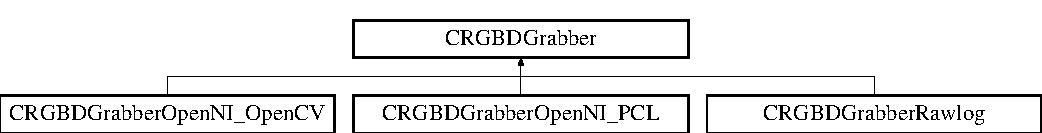
\includegraphics[height=1.786284cm]{class_c_r_g_b_d_grabber}
\end{center}
\end{figure}
\subsection*{Public Member Functions}
\begin{DoxyCompactItemize}
\item 
virtual void \hyperlink{class_c_r_g_b_d_grabber_ab1aa7a5c871104dd8791d5a3a5117e3a}{init} ()=0
\item 
virtual void \hyperlink{class_c_r_g_b_d_grabber_aa7f9c715a16933287a92ecaf7a1bbfb4}{grab} (\hyperlink{class_c_frame_r_g_b_d}{CFrameRGBD} $\ast$)=0
\item 
virtual void \hyperlink{class_c_r_g_b_d_grabber_a653ef16978adcd9000079f0e5f00addc}{stop} ()=0
\end{DoxyCompactItemize}
\subsection*{Protected Attributes}
\begin{DoxyCompactItemize}
\item 
\hyperlink{class_c_frame_r_g_b_d}{CFrameRGBD} $\ast$ \hyperlink{class_c_r_g_b_d_grabber_a672772dade93a640a52e129f14c6d2fa}{framePtr}
\end{DoxyCompactItemize}


\subsection{Detailed Description}
Abstract class that especifies the functionality of a generic RGBD grabber. 

\subsection{Member Function Documentation}
\hypertarget{class_c_r_g_b_d_grabber_aa7f9c715a16933287a92ecaf7a1bbfb4}{
\index{CRGBDGrabber@{CRGBDGrabber}!grab@{grab}}
\index{grab@{grab}!CRGBDGrabber@{CRGBDGrabber}}
\subsubsection[{grab}]{\setlength{\rightskip}{0pt plus 5cm}virtual void CRGBDGrabber::grab (
\begin{DoxyParamCaption}
\item[{{\bf CFrameRGBD} $\ast$}]{}
\end{DoxyParamCaption}
)\hspace{0.3cm}{\ttfamily  \mbox{[}pure virtual\mbox{]}}}}
\label{class_c_r_g_b_d_grabber_aa7f9c715a16933287a92ecaf7a1bbfb4}
Retains the current RGBD frame. 

Implemented in \hyperlink{class_c_r_g_b_d_grabber_open_n_i___open_c_v_a7a1d5c1d4ec74000b15d60e0683d9e77}{CRGBDGrabberOpenNI\_\-OpenCV}, \hyperlink{class_c_r_g_b_d_grabber_open_n_i___p_c_l_ab01be725fe3388898a9bad48aa6e15bb}{CRGBDGrabberOpenNI\_\-PCL}, and \hyperlink{class_c_r_g_b_d_grabber_rawlog_a22e26394c6f7d83d45c5de01a4c999b4}{CRGBDGrabberRawlog}.

\hypertarget{class_c_r_g_b_d_grabber_ab1aa7a5c871104dd8791d5a3a5117e3a}{
\index{CRGBDGrabber@{CRGBDGrabber}!init@{init}}
\index{init@{init}!CRGBDGrabber@{CRGBDGrabber}}
\subsubsection[{init}]{\setlength{\rightskip}{0pt plus 5cm}virtual void CRGBDGrabber::init (
\begin{DoxyParamCaption}
{}
\end{DoxyParamCaption}
)\hspace{0.3cm}{\ttfamily  \mbox{[}pure virtual\mbox{]}}}}
\label{class_c_r_g_b_d_grabber_ab1aa7a5c871104dd8791d5a3a5117e3a}
Initializes the grabber object 

Implemented in \hyperlink{class_c_r_g_b_d_grabber_open_n_i___open_c_v_ac3f36ad66da25fb590e915072bece32e}{CRGBDGrabberOpenNI\_\-OpenCV}, \hyperlink{class_c_r_g_b_d_grabber_open_n_i___p_c_l_abffd24f81fc9d0668ade3fae4a610a5b}{CRGBDGrabberOpenNI\_\-PCL}, and \hyperlink{class_c_r_g_b_d_grabber_rawlog_abf3ace5b3c3fbc947b47a0caec76791d}{CRGBDGrabberRawlog}.

\hypertarget{class_c_r_g_b_d_grabber_a653ef16978adcd9000079f0e5f00addc}{
\index{CRGBDGrabber@{CRGBDGrabber}!stop@{stop}}
\index{stop@{stop}!CRGBDGrabber@{CRGBDGrabber}}
\subsubsection[{stop}]{\setlength{\rightskip}{0pt plus 5cm}virtual void CRGBDGrabber::stop (
\begin{DoxyParamCaption}
{}
\end{DoxyParamCaption}
)\hspace{0.3cm}{\ttfamily  \mbox{[}pure virtual\mbox{]}}}}
\label{class_c_r_g_b_d_grabber_a653ef16978adcd9000079f0e5f00addc}
Stop grabing RGBD frames. 

Implemented in \hyperlink{class_c_r_g_b_d_grabber_open_n_i___open_c_v_a3a16ce107e7d613fef517096f3dff39f}{CRGBDGrabberOpenNI\_\-OpenCV}, \hyperlink{class_c_r_g_b_d_grabber_open_n_i___p_c_l_a7ed8695258084e50b76241fe8543f527}{CRGBDGrabberOpenNI\_\-PCL}, and \hyperlink{class_c_r_g_b_d_grabber_rawlog_af499a26d2f6a92184fcc457e9c664da3}{CRGBDGrabberRawlog}.



\subsection{Field Documentation}
\hypertarget{class_c_r_g_b_d_grabber_a672772dade93a640a52e129f14c6d2fa}{
\index{CRGBDGrabber@{CRGBDGrabber}!framePtr@{framePtr}}
\index{framePtr@{framePtr}!CRGBDGrabber@{CRGBDGrabber}}
\subsubsection[{framePtr}]{\setlength{\rightskip}{0pt plus 5cm}{\bf CFrameRGBD}$\ast$ {\bf CRGBDGrabber::framePtr}\hspace{0.3cm}{\ttfamily  \mbox{[}protected\mbox{]}}}}
\label{class_c_r_g_b_d_grabber_a672772dade93a640a52e129f14c6d2fa}
Pointer to the last grabbed RGBD frame 

The documentation for this class was generated from the following file:\begin{DoxyCompactItemize}
\item 
CRGBDGrabber.h\end{DoxyCompactItemize}

\hypertarget{class_c_r_g_b_d_grabber_rawlog}{
\section{CRGBDGrabberRawlog Class Reference}
\label{class_c_r_g_b_d_grabber_rawlog}\index{CRGBDGrabberRawlog@{CRGBDGrabberRawlog}}
}


{\ttfamily \#include $<$CRGBDGrabberRawlog.h$>$}

Inheritance diagram for CRGBDGrabberRawlog:\begin{figure}[H]
\begin{center}
\leavevmode
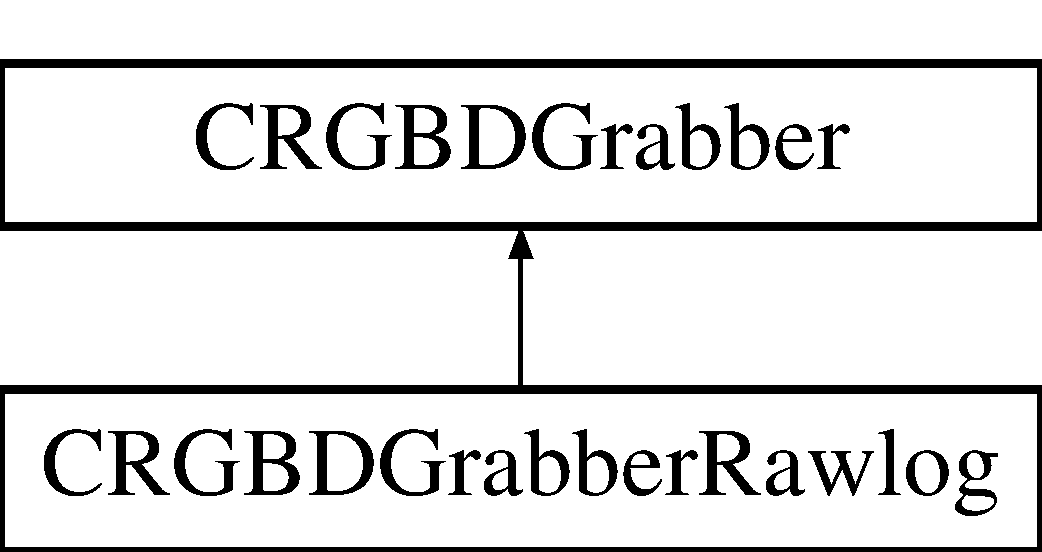
\includegraphics[height=2.000000cm]{class_c_r_g_b_d_grabber_rawlog}
\end{center}
\end{figure}
\subsection*{Public Member Functions}
\begin{DoxyCompactItemize}
\item 
\hyperlink{class_c_r_g_b_d_grabber_rawlog_aabfd5bddf00ddb3a43d0a13280c32c24}{CRGBDGrabberRawlog} (const std::string \&rawlog\_\-file)
\item 
void \hyperlink{class_c_r_g_b_d_grabber_rawlog_abf3ace5b3c3fbc947b47a0caec76791d}{init} ()
\item 
void \hyperlink{class_c_r_g_b_d_grabber_rawlog_a22e26394c6f7d83d45c5de01a4c999b4}{grab} (\hyperlink{class_c_frame_r_g_b_d}{CFrameRGBD} $\ast$)
\item 
void \hyperlink{class_c_r_g_b_d_grabber_rawlog_af499a26d2f6a92184fcc457e9c664da3}{stop} ()
\end{DoxyCompactItemize}
\subsection*{Private Attributes}
\begin{DoxyCompactItemize}
\item 
\hypertarget{class_c_r_g_b_d_grabber_rawlog_a1a90df6d545fdd0cce5da3d4e48d3700}{
mrpt::slam::CObservation3DRangeScanPtr {\bfseries currentObservationPtr}}
\label{class_c_r_g_b_d_grabber_rawlog_a1a90df6d545fdd0cce5da3d4e48d3700}

\item 
\hypertarget{class_c_r_g_b_d_grabber_rawlog_a9ead576a05025c9c3f59dde0b23d8be6}{
mrpt::utils::CFileGZInputStream $\ast$ {\bfseries dataset}}
\label{class_c_r_g_b_d_grabber_rawlog_a9ead576a05025c9c3f59dde0b23d8be6}

\item 
\hypertarget{class_c_r_g_b_d_grabber_rawlog_add51cd2527e3d5ca829a25119b75f71e}{
bool {\bfseries endGrabbing}}
\label{class_c_r_g_b_d_grabber_rawlog_add51cd2527e3d5ca829a25119b75f71e}

\item 
\hypertarget{class_c_r_g_b_d_grabber_rawlog_a33406069d1bf46517105224d63e2c994}{
uint64\_\-t {\bfseries lastTimestamp}}
\label{class_c_r_g_b_d_grabber_rawlog_a33406069d1bf46517105224d63e2c994}

\end{DoxyCompactItemize}


\subsection{Detailed Description}
This class captures RGBD frames from rawlog sensor data using the MRPT library. It grabs the intensity image as well as its depth image. It also grabs the timestamp of each frame if provided in the rawlog. 

\subsection{Constructor \& Destructor Documentation}
\hypertarget{class_c_r_g_b_d_grabber_rawlog_aabfd5bddf00ddb3a43d0a13280c32c24}{
\index{CRGBDGrabberRawlog@{CRGBDGrabberRawlog}!CRGBDGrabberRawlog@{CRGBDGrabberRawlog}}
\index{CRGBDGrabberRawlog@{CRGBDGrabberRawlog}!CRGBDGrabberRawlog@{CRGBDGrabberRawlog}}
\subsubsection[{CRGBDGrabberRawlog}]{\setlength{\rightskip}{0pt plus 5cm}CRGBDGrabberRawlog::CRGBDGrabberRawlog (
\begin{DoxyParamCaption}
\item[{const std::string \&}]{rawlog\_\-file}
\end{DoxyParamCaption}
)}}
\label{class_c_r_g_b_d_grabber_rawlog_aabfd5bddf00ddb3a43d0a13280c32c24}
Creates a \hyperlink{class_c_r_g_b_d_grabber_rawlog}{CRGBDGrabberRawlog} instance that grabs RGBD frames from the specified rawlog file. 

\subsection{Member Function Documentation}
\hypertarget{class_c_r_g_b_d_grabber_rawlog_a22e26394c6f7d83d45c5de01a4c999b4}{
\index{CRGBDGrabberRawlog@{CRGBDGrabberRawlog}!grab@{grab}}
\index{grab@{grab}!CRGBDGrabberRawlog@{CRGBDGrabberRawlog}}
\subsubsection[{grab}]{\setlength{\rightskip}{0pt plus 5cm}void CRGBDGrabberRawlog::grab (
\begin{DoxyParamCaption}
\item[{{\bf CFrameRGBD} $\ast$}]{}
\end{DoxyParamCaption}
)\hspace{0.3cm}{\ttfamily  \mbox{[}virtual\mbox{]}}}}
\label{class_c_r_g_b_d_grabber_rawlog_a22e26394c6f7d83d45c5de01a4c999b4}
Retains the current RGBD frame. 

Implements \hyperlink{class_c_r_g_b_d_grabber_aa7f9c715a16933287a92ecaf7a1bbfb4}{CRGBDGrabber}.

\hypertarget{class_c_r_g_b_d_grabber_rawlog_abf3ace5b3c3fbc947b47a0caec76791d}{
\index{CRGBDGrabberRawlog@{CRGBDGrabberRawlog}!init@{init}}
\index{init@{init}!CRGBDGrabberRawlog@{CRGBDGrabberRawlog}}
\subsubsection[{init}]{\setlength{\rightskip}{0pt plus 5cm}void CRGBDGrabberRawlog::init (
\begin{DoxyParamCaption}
{}
\end{DoxyParamCaption}
)\hspace{0.3cm}{\ttfamily  \mbox{[}inline, virtual\mbox{]}}}}
\label{class_c_r_g_b_d_grabber_rawlog_abf3ace5b3c3fbc947b47a0caec76791d}
Initializes the grabber object 

Implements \hyperlink{class_c_r_g_b_d_grabber_ab1aa7a5c871104dd8791d5a3a5117e3a}{CRGBDGrabber}.

\hypertarget{class_c_r_g_b_d_grabber_rawlog_af499a26d2f6a92184fcc457e9c664da3}{
\index{CRGBDGrabberRawlog@{CRGBDGrabberRawlog}!stop@{stop}}
\index{stop@{stop}!CRGBDGrabberRawlog@{CRGBDGrabberRawlog}}
\subsubsection[{stop}]{\setlength{\rightskip}{0pt plus 5cm}void CRGBDGrabberRawlog::stop (
\begin{DoxyParamCaption}
{}
\end{DoxyParamCaption}
)\hspace{0.3cm}{\ttfamily  \mbox{[}inline, virtual\mbox{]}}}}
\label{class_c_r_g_b_d_grabber_rawlog_af499a26d2f6a92184fcc457e9c664da3}
Stop grabing RGBD frames. 

Implements \hyperlink{class_c_r_g_b_d_grabber_a653ef16978adcd9000079f0e5f00addc}{CRGBDGrabber}.



The documentation for this class was generated from the following file:\begin{DoxyCompactItemize}
\item 
CRGBDGrabberRawlog.h\end{DoxyCompactItemize}

\hypertarget{class_point_cloud_downsampler}{
\section{PointCloudDownsampler Class Reference}
\label{class_point_cloud_downsampler}\index{PointCloudDownsampler@{PointCloudDownsampler}}
}


{\ttfamily \#include $<$PointCloudDownsampler.h$>$}

\subsection*{Public Member Functions}
\begin{DoxyCompactItemize}
\item 
\hyperlink{class_point_cloud_downsampler_a518e890b357eed74601e0fc940334343}{PointCloudDownsampler} (const int=8)
\item 
void \hyperlink{class_point_cloud_downsampler_aa59d5affe32288f96dd2ac1ff46aab35}{setDownsamplingStep} (const int)
\item 
void \hyperlink{class_point_cloud_downsampler_a6c2648119f30b8c41c5851844c1acb29}{downsamplePointCloud} (pcl::PointCloud$<$ pcl::PointXYZRGBA $>$::Ptr pointCloudPtr, pcl::PointCloud$<$ pcl::PointXYZRGBA $>$::Ptr downsampledPointCloudPtr)
\item 
void \hyperlink{class_point_cloud_downsampler_aa974584d15d1de898bbec8dbf791b29f}{downsamplePointCloudColor} (pcl::PointCloud$<$ pcl::PointXYZRGBA $>$::Ptr, pcl::PointCloud$<$ pcl::PointXYZRGBA $>$::Ptr)
\end{DoxyCompactItemize}
\subsection*{Private Attributes}
\begin{DoxyCompactItemize}
\item 
\hypertarget{class_point_cloud_downsampler_a74b48c9180a5d63ab550e26f07c24df0}{
int {\bfseries downsamplingStep}}
\label{class_point_cloud_downsampler_a74b48c9180a5d63ab550e26f07c24df0}

\end{DoxyCompactItemize}


\subsection{Detailed Description}
This class implements a fast and straightforward algorithm to downsample organized 3D point clouds. The algorithm takes the median point of a square region (downsamplingStep x downsamplingStep) of 3D points to mitigate the data noise. 

\subsection{Constructor \& Destructor Documentation}
\hypertarget{class_point_cloud_downsampler_a518e890b357eed74601e0fc940334343}{
\index{PointCloudDownsampler@{PointCloudDownsampler}!PointCloudDownsampler@{PointCloudDownsampler}}
\index{PointCloudDownsampler@{PointCloudDownsampler}!PointCloudDownsampler@{PointCloudDownsampler}}
\subsubsection[{PointCloudDownsampler}]{\setlength{\rightskip}{0pt plus 5cm}PointCloudDownsampler::PointCloudDownsampler (
\begin{DoxyParamCaption}
\item[{const int}]{ = {\ttfamily 8}}
\end{DoxyParamCaption}
)}}
\label{class_point_cloud_downsampler_a518e890b357eed74601e0fc940334343}
Constructor of an instance of \hyperlink{class_point_cloud_downsampler}{PointCloudDownsampler} given the downsamplingStep 

\subsection{Member Function Documentation}
\hypertarget{class_point_cloud_downsampler_a6c2648119f30b8c41c5851844c1acb29}{
\index{PointCloudDownsampler@{PointCloudDownsampler}!downsamplePointCloud@{downsamplePointCloud}}
\index{downsamplePointCloud@{downsamplePointCloud}!PointCloudDownsampler@{PointCloudDownsampler}}
\subsubsection[{downsamplePointCloud}]{\setlength{\rightskip}{0pt plus 5cm}void PointCloudDownsampler::downsamplePointCloud (
\begin{DoxyParamCaption}
\item[{pcl::PointCloud$<$ pcl::PointXYZRGBA $>$::Ptr}]{pointCloudPtr, }
\item[{pcl::PointCloud$<$ pcl::PointXYZRGBA $>$::Ptr}]{downsampledPointCloudPtr}
\end{DoxyParamCaption}
)}}
\label{class_point_cloud_downsampler_a6c2648119f30b8c41c5851844c1acb29}
Downsamples the point cloud given by pointCloudPtr skiping the RGB information. The resulting downsampled point cloud is returned in downsampledPointCloudPtr. \hypertarget{class_point_cloud_downsampler_aa974584d15d1de898bbec8dbf791b29f}{
\index{PointCloudDownsampler@{PointCloudDownsampler}!downsamplePointCloudColor@{downsamplePointCloudColor}}
\index{downsamplePointCloudColor@{downsamplePointCloudColor}!PointCloudDownsampler@{PointCloudDownsampler}}
\subsubsection[{downsamplePointCloudColor}]{\setlength{\rightskip}{0pt plus 5cm}void PointCloudDownsampler::downsamplePointCloudColor (
\begin{DoxyParamCaption}
\item[{pcl::PointCloud$<$ pcl::PointXYZRGBA $>$::Ptr}]{, }
\item[{pcl::PointCloud$<$ pcl::PointXYZRGBA $>$::Ptr}]{}
\end{DoxyParamCaption}
)}}
\label{class_point_cloud_downsampler_aa974584d15d1de898bbec8dbf791b29f}
Downsamples the point cloud given by pointCloudPtr. The color information will be computed by taking the median RGB value in the square region. The resulting downsampled point cloud is returned in downsampledPointCloudPtr. \hypertarget{class_point_cloud_downsampler_aa59d5affe32288f96dd2ac1ff46aab35}{
\index{PointCloudDownsampler@{PointCloudDownsampler}!setDownsamplingStep@{setDownsamplingStep}}
\index{setDownsamplingStep@{setDownsamplingStep}!PointCloudDownsampler@{PointCloudDownsampler}}
\subsubsection[{setDownsamplingStep}]{\setlength{\rightskip}{0pt plus 5cm}void PointCloudDownsampler::setDownsamplingStep (
\begin{DoxyParamCaption}
\item[{const int}]{}
\end{DoxyParamCaption}
)}}
\label{class_point_cloud_downsampler_aa59d5affe32288f96dd2ac1ff46aab35}
Sets the desired downsamplingStep to the given value 

The documentation for this class was generated from the following file:\begin{DoxyCompactItemize}
\item 
PointCloudDownsampler.h\end{DoxyCompactItemize}

\hypertarget{class_photoconsistency_odometry_1_1_ceres_1_1_c_photoconsistency_odometry_ceres_1_1_residual_r_g_b_d_photoconsistency}{
\section{PhotoconsistencyOdometry::Ceres::CPhotoconsistencyOdometryCeres::ResidualRGBDPhotoconsistency Class Reference}
\label{class_photoconsistency_odometry_1_1_ceres_1_1_c_photoconsistency_odometry_ceres_1_1_residual_r_g_b_d_photoconsistency}\index{PhotoconsistencyOdometry::Ceres::CPhotoconsistencyOdometryCeres::ResidualRGBDPhotoconsistency@{PhotoconsistencyOdometry::Ceres::CPhotoconsistencyOdometryCeres::ResidualRGBDPhotoconsistency}}
}
\subsection*{Public Member Functions}
\begin{DoxyCompactItemize}
\item 
\hypertarget{class_photoconsistency_odometry_1_1_ceres_1_1_c_photoconsistency_odometry_ceres_1_1_residual_r_g_b_d_photoconsistency_a2a16cbc3f15bb2e3232c29b66fd313ed}{
{\footnotesize template$<$typename T $>$ }\\bool {\bfseries operator()} (const T $\ast$const stateVector, T $\ast$residuals) const }
\label{class_photoconsistency_odometry_1_1_ceres_1_1_c_photoconsistency_odometry_ceres_1_1_residual_r_g_b_d_photoconsistency_a2a16cbc3f15bb2e3232c29b66fd313ed}

\end{DoxyCompactItemize}


The documentation for this class was generated from the following file:\begin{DoxyCompactItemize}
\item 
CPhotoconsistencyOdometryCeres.h\end{DoxyCompactItemize}

\hypertarget{class_photoconsistency_odometry_1_1_ceres_1_1_c_photoconsistency_odometry_ceres_1_1_visualization_callback}{
\section{PhotoconsistencyOdometry::Ceres::CPhotoconsistencyOdometryCeres::VisualizationCallback Class Reference}
\label{class_photoconsistency_odometry_1_1_ceres_1_1_c_photoconsistency_odometry_ceres_1_1_visualization_callback}\index{PhotoconsistencyOdometry::Ceres::CPhotoconsistencyOdometryCeres::VisualizationCallback@{PhotoconsistencyOdometry::Ceres::CPhotoconsistencyOdometryCeres::VisualizationCallback}}
}
\subsection*{Public Member Functions}
\begin{DoxyCompactItemize}
\item 
\hypertarget{class_photoconsistency_odometry_1_1_ceres_1_1_c_photoconsistency_odometry_ceres_1_1_visualization_callback_a6b6ca449fe52592c14d9160e1228d2e5}{
virtual ceres::CallbackReturnType {\bfseries operator()} (const ceres::IterationSummary \&summary)}
\label{class_photoconsistency_odometry_1_1_ceres_1_1_c_photoconsistency_odometry_ceres_1_1_visualization_callback_a6b6ca449fe52592c14d9160e1228d2e5}

\end{DoxyCompactItemize}


The documentation for this class was generated from the following file:\begin{DoxyCompactItemize}
\item 
CPhotoconsistencyOdometryCeres.h\end{DoxyCompactItemize}

\printindex
\end{document}
